\documentclass[class=book, crop=false, oneside, 12pt]{standalone}
\usepackage{standalone}
\usepackage{../../style}
\usepackage[normalem]{ulem}
\graphicspath{{./assets/images/}}

% arara: pdflatex: { synctex: yes, shell: yes }
% arara: latexmk: { clean: partial }
\begin{document}
\chapter{Analisi semantica}

\section{Introduzione all'analisi semantica}

\subsection{Grammatiche attribuite}
Nei capitoli precedenti abbiamo trattato esaustivamente la fase dell'analisi sintattica, in questo capitolo è finalmente arrivato il momento di passare all'analisi semantica.

Per approcciarsi a questa fase del processo della compilazione è necessario introdurre il concetto di grammatica attribuita (Syntax-Directed Definitions, da ora in poi SDD).

Questo tipo di grammatica è tale e quale ad una grammatica di quelle che siamo abituati ad utilizzare ormai quotidianamente, ma ci sorprende con due elementi aggiuntivi:
\begin{itemize}
    \item \textbf{Attributi} che sono associati ai simboli della grammatica e possono essere numeri, tipi, riferimenti alla tabella dei simboli ecc; 
    \item \textbf{Regole} che sono associate alle produzioni della grammatica e di norma sono funzioni degli attributi dei simboli della produzione.
\end{itemize}
Sia simboli che regole sono utilizzati per compiere l'analisi semantica, ovvero dare un valore a quello che è espresso da una parola di un a certa grammatica.

\subsection{Tipi di attributi}

Gli attributi sono divisi in due categorie:
\begin{itemize}
    \item \textbf{attributi sintetizzati}, sono gli attributi del driver di una produzione, questi sono definiti in funzione degli attributi dei simboli del body della produzione;
    \item \textbf{attributi ereditati}, sono gli attributi dei non-terminali nel body della produzione e sono definiti in funzione degli altri simboli del body della produzione.
\end{itemize}
Il lettore accorto si sarà reso cont senz'altro che non abbiamo definito degli attributi per i caratteri terminali, questo perché gli attributi dei terminali sono sempre noti: sono dati dall'analisi lessicale e di conseguenza non serve alcuna regola per calcolarli.
Questo concetto risulta più chiaro se si tiene bene a mente che gli attributi servono per valorizzare i caratteri di una parola: i non-terminali hanno un valore che dipende da che funzione rappresentano e da quali terminali "utilizzano", i terminali invece rappresentano le variabili, ovvero dei valori ben definiti che sono già stati riconosciuti e salvati nel momento dell'analisi lessicale.

Di fatto l'analizzatore lessicale prende il codice, sostituisce i terminali con i loro identificatori e ne memorizza il valore.
L'analizzatore lessicale passa poi all'analizzatore sintattico la tabella dei simboli in cui ogni identificatore ha associato il suo valore lessicale (che in seguito indicheremo con la keyword \texttt{lexval}).

È arrivato, come da prassi, il momento di applicare la nostra filosofia del \emph{learning by doing}, osservando un esempio di utilizzo di una grammatica attribuita.

\subsection{Esempio}
Prendiamo come esempio la nostra grammatica per la valutazione delle espressioni aritmetiche per valutare l'espressione rappresentata dall'albero di derivazione in Fig.\ref{fig:first-ex_SDD}.
\begin{align*}
    V &\to E \\
    E &\to E + T \mid T\\
    T &\to T * F \mid F\\
    F &\to (E) \mid digit
\end{align*}
\begin{figure}[H]
    \centering
    \includegraphics[width=.8\textwidth]{first-ex_SDD.jpg}
    \caption{Albero di derivazione per una somma}
    \label{fig:first-ex_SDD}
\end{figure}
Prendiamo il caso in cui il primo digit abbia assegnato come valore 3, mentre il secondo abbia valore 4.
Questi valori, come spiegato prima, sono memorizzati nella tabella dei simboli.

Naturalmente essendo questa una somma tra 3 e 4 ci aspettiamo di trovare, una volta terminata la fase di valutazione, che il valore riportato in \(V\) sia 7.

Vediamo subito quale forma deve avere l'SDD per la grammatica che stiamo utilizzando:
\begin{align}
    \label{reg:regola-1}
    V &\to E & &\{V.val = E.val\} \\
    \label{reg:regola-2}
    E &\to E_1 + T & &\{E.val = E_1.val + T.val\} \\
    \label{reg:regola-3}
    E &\to T & &\{E.val = T.val\} \\
    \label{reg:regola-4}
    T &\to T_1 * F & &\{T.val = T_1.val * F.val\} \\
    \label{reg:regola-5}
    T &\to F & &\{T.val = F.val\} \\
    \label{reg:regola-6}
    F &\to (E) & &\{F.val = E.val\} \\
    \label{reg:regola-7}
    F &\to digit & &\{F.val = digit.lexval\}
\end{align}
Nota che i pedici numerici usati in alcune produzioni sono usati solo per differenziare il body dal driver, non hanno nessuna valenza semantica, di fatto \(E_1\) ed \(E\) sono lo stesso non-terminale.

\paragraph*{Significato delle regole} quelle che abbiamo elencato sulla destra delle produzioni tra parentesi giraffe sono le regole che compongono una grammatica attribuita.

\noindent Tutto ciò che si trova all'interno delle regole sono gli attributi (nota però che i simboli + e \(*\) in questo caso non sono attributi, ma sono proprio le operazioni matematiche).

\noindent Proviamo ora a dare una spiegazione del significato delle varie regole così da aiutare il lettore a capire meglio qual è lo scopo delle grammatiche attribuite.
\begin{itemize}
    \item[Reg.\ref{reg:regola-1}] la prima produzione è una produzione aggiuntiva che abbiamo inserito noi  (un po' come \(S' \to S\)) e ci dice che quando incontriamo produzioni \(V \to E\) il valore di \(V\) è \(E.val\);
    \item[Reg.\ref{reg:regola-2}] per produzioni come \(E \to E_1 + T\) avremo che il valore di \(E\) corrisponde alla somma del sottoalbero \(E_1\) più il valore di \(T\) (nota che \(E_1\) è usato solo per differenziare da \(E\));
    \item[Reg.\ref{reg:regola-3}] se ho una produzione \(E \to T\) il valore di \(E\) è uguale al valore di \(T\);
    \item[Reg.\ref{reg:regola-4}] se ho una produzione \(T\to T_1 * F\) il valore di \(T\) corrisponde al valore del sottoalbero \(T_1\) moltiplicato per il valore di \(F\) (nota che \(T_1\) è usato solo per differenziare da \(T\));
    \item[Reg.\ref{reg:regola-5}] se ho una produzione del tipo \(T\to F\) il valore di \(T\) è uguale a \(F.val\);
    \item[Reg.\ref{reg:regola-6}] se ho una produzione del tipo \(F \to (E)\) il valore che assegno a \(F\) corrisponde a \(E.val\);
    \item[Reg.\ref{reg:regola-7}] se ho una produzione del tipo \(F \to digit\) mi aspetto che il valore di \(F\) sia il valore riportato nella tabella dei simboli per tale \(digit\).
\end{itemize}

\paragraph*{Utilizzo dell'SDD} Ora che abbiamo la grammatica attribuita possiamo utilizzarla appunto per dare un valore al parse tree della nostra somma.

Per valutare un albero di derivazione si utilizza un parse tree annotato. Questo è un parse tree in cui ogni nodo contiene le annotazioni che riguardano gli attributi del simbolo che si trova in quel nodo.
Si può capire al volo cosa intendiamo guardando il parse tree annotato corrispondente al parse tree precedente (Fig.\ref{fig:first-ex_SDD})) che è raffigurato qui sotto.
\begin{figure}[H]
    \centering
    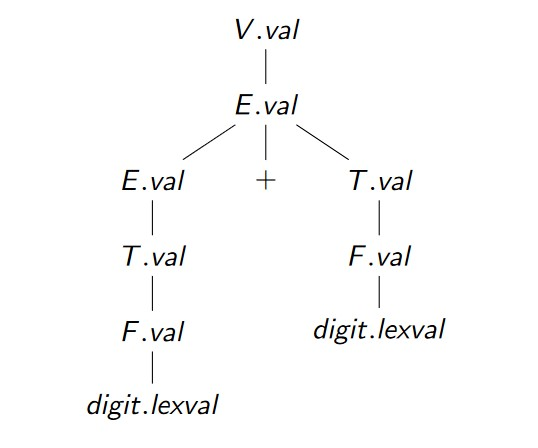
\includegraphics[width=.8\textwidth]{first-ex_noted-parse-tree.jpg}
    \caption{Parse tree annoiato per la somma in \ref{fig:first-ex_SDD}}
    \label{fig:first-ex_noted-parse-tree}
\end{figure}
Ciò a cui si deve fare attenzione in questo caso è che ad ogni nodo è aggiunta l'annotazione riguardante il valore del nodo stesso.

Ma a cosa serve il parse tree annotato? È presto detto!

\noindent Il parse tree annotato viene letto dal basso verso l'alto seguendo le regole di attribuzione che sono segnate sui vari nodi per ottenere la valutazione dell'albero stesso. Vediamo ora questo procedimento passo per passo.

\begin{enumerate}
    \item Partendo dal basso applichiamo innanzitutto la regola
    \begin{align*}
        F &\to digit & &\{F.val = digit.lexval\}
    \end{align*}
    \begin{figure}[H]
        \centering
        \includegraphics[width=.5\textwidth]{first-ex_SDD-resolution-step-1.jpg}
        \caption{Passo 1 della valutazione tramite SDD}
    \end{figure}
    \item Il secondo passo prevede di applicare la regola
    \begin{align*}
        T &\to F & &\{T.val = F.val\}
    \end{align*}
    \begin{figure}[H]
        \centering
        \includegraphics[width=.5\textwidth]{first-ex_SDD-resolution-step-2.jpg}
        \caption{Passo 2 della valutazione tramite SDD}
    \end{figure}
    \item Successivamente applichiamo la regola
    \begin{align*}
        E &\to T & &\{E.val = T.val\}
    \end{align*}
    \begin{figure}[H]
        \centering
        \includegraphics[width=.5\textwidth]{first-ex_SDD-resolution-step-3.jpg}
        \caption{Passo 3 della valutazione tramite SDD}
    \end{figure}
    \item Il quarto passo prevede di applicare la regola
    \begin{align*}
        E &\to E_1 + T & &\{E.val = E_1.val + T.val\}
    \end{align*}
    \begin{figure}[H]
        \centering
        \includegraphics[width=.5\textwidth]{first-ex_SDD-resolution-step-4.jpg}
        \caption{Passo 4 della valutazione tramite SDD}
    \end{figure}
    \item Infine, andiamo ad applicare la regola
    \begin{align*}
        V &\to E & &\{V.val = E.val\}
    \end{align*}
    \begin{figure}[H]
        \centering
        \includegraphics[width=.5\textwidth]{first-ex_SDD-resolution-step-5.jpg}
        \caption{Passo finale della valutazione tramite SDD}
    \end{figure}
\end{enumerate}
Dovrebbe essere chiaro a questo punto come si possa utilizzare una grammatica attribuita per calcolare il valore di una certa parola di una data grammatica:
\begin{enumerate}
    \item si crea il parse tree annotato per tale parola;
    \item si utilizza il parse tree annotato in combinazione con le regole dettate dalla grammatica attribuita per valorizzare un nodo alla volta tutti i nodi del parse tree annotato;
    \item una volta valorizzata la radice del parse tree annotato si è ricavato il valore della parola.
\end{enumerate}
Una nota interessante riguardo all'albero di parsing annotato visto in questo esempio è che gli attributi che compaiono in tutti i nodi sono attributi sintetizzati.

\subsection{Verificare se un parse tree annotato può essere valutato}
Non è sempre detto che un parse tree annotato possa essere valutato, per verificare che ciò sia possibile dobbiamo utilizziare un grafo delle dipendenze e verificare che non vi siano conflitti tra le dipendenze.

\paragraph*{Costruire il grafo delle dipendenze} per definire un grafo delle dipendenze per un determinato parse tree annotato dobbiamo svolgere i seguenti passi:

\begin{itemize}
    \item impostiamo un nodo nel grafo delle dipendenze per ogni attributo associato a qualche nodo del parse tree;
    \item per ogni attributo \(X.x\) usato per definire l'attributo \(Y.y\), creiamo un arco dal nodo di \(X.x\) fino al nodo di \(Y.y\) (rappresentando quindi la dipendenza di \(Y.y\) da \(X.x\)).
\end{itemize}

\paragraph*{Utilizzare il grafo delle dipendenze} una volta creato il grafo delle dipendenze, per verificare che non vi siano conflitti dobbiamo trovare un ordinamento topologico per tale grafo; se un ordinamento topologico non esiste, allora l'albero di parsing annotato non è valutabile.

\noindent Se invece troviamo un ordinamento topologico per questo dependency graph allora l'SDD è valutabile ed abbiamo anche un ordine da seguire per la valutazione.

Ad esempio per il parse tree annotato dell'esercizio precedente otteniamo questo grafo delle dipendenze in cui le dipendenze sono indicate con le frecce azzurre (mentre la linea tratteggiata rappresenta gli archi del parse tree).
\begin{figure}[H]
    \centering
    \includegraphics[width=.8\textwidth]{first-ex_SDD-dependency-graph.jpg}
    \caption{Albero di parsing annotato e relativo grafo delle dipendenze}
    \label{fig:first-ex_SDD-dependency-graph}
\end{figure}
In generale vale questa regola: quando tutti gli attributi sono di tipo sintetizzato allora una visita in postordine può sostituire sempre l'ordinamento topologico, capiremo in seguito le motivazioni dietro questa affermazione.

Riportiamo lo pseudocodice della visita in postordine, per chi non avesse ascoltato il Montre a suo tempo:
\begin{figure}[H]
    \centering
    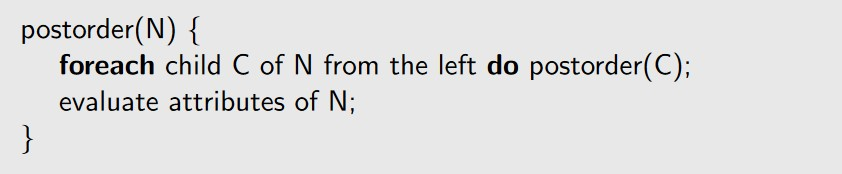
\includegraphics[width=.8\textwidth]{postorder-visit.jpg}
    \caption{Algoritmo della visita in postordine, versione PQ}
    \label{fig:postorder-visit}
\end{figure}
Quando un SDD contiene sia elementi sintetizzati che ereditati allora non c'è la garanzia che un ordinamento topologico esista per tale SDD.
Per esempio, se si ha una regola come 
\begin{align*}
    A &\to B & & &\{A.s = B.i; B.i = A.s+7\} 
\end{align*}
si potrebbe trovare un ciclo all'interno del grafo delle dipendenze con una forma simile:
\begin{figure}[H]
    \centering
    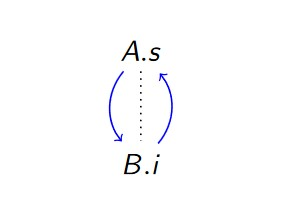
\includegraphics[width=.5\textwidth]{dependence-conflict.jpg}
    \caption{Conflitto di dipendenza}
    \label{fig:dependence-conflict}
\end{figure}
Quindi nel caso generale si calcola sempre l'ordinamento topologico dell'SDD, solo nel caso specifico di SDD costituiti solo da attributi sintetizzati ci basta la visita in postordine (che in questo caso corrisponde proprio ad un ordinamento topologico).

Esistono due classi di SDD per cui è sempre garantita l'esistenza di un ordinamento topologico:
\begin{itemize}
    \item \textbf{S-attributed SDD} (grammatiche o SDD s-attribuiti): tutti gli attributi dell'SDD sono sintetizzati, in questo caso come già detto ci basta fare una visita in postordine;
    \item \textbf{L-attributed SDD}: ci possono essere anche attributi ereditati che rispettano però il seguente vincolo sulle eredità: si può ereditare solo dal padre o dai fratelli sinistri; scrivendo in linguaggio matematico tale vincolo:
    \begin{itemize}
        \item per ogni produzione \(A \to X_1 ... X_n\) la definizione di ogni \(X_j.i\) utilizza solamente
        \begin{itemize}
            \item attributi ereditati di A oppure
            \item attributi sintetizzati o ereditati dei fratelli sinistri di \(X_j\), ovvero \(X_1 ... X_{j-1}\)
        \end{itemize}
    \end{itemize}
\end{itemize}
Gli SDD S-attribuiti sono ideali per il parsing bottom-up, perché si può creare e valutare il parse tree attribuito in contemporanea al parsing della stringa.

\noindent Viceversa gli SDD L-attribuiti sono invece ideali per il parsing top-down, perché si può creare e valutare il parsing tree attribuito in contemporanea al parsing della stringa.

\subsection{Un altro esempio di utilizzo dell'SDD}
Grammatiche differenti pongono sfide differenti nella definizione degli SDD.
Nel primo esercizio di applicazione dell'SDD abbiamo studiato una grammatica con ricorsione sinistra, osserviamo ora un caso di grammatica LL(1), consideriamo il caso della grammatica per le espressioni aritmetiche \(+\) e \(*\).
\begin{align*}
    V &\to E \\
    E &\to TE' \\
    E' &\to +TE \mid \varepsilon \\
    T &\to FT' \\
    T' &\to *FT' \mid \varepsilon \\
    F &\to (E) \mid digit \\
\end{align*}
Volgiamo definire l'SDD che ci permette di valutare tale grammatica.

Vediamo di costruire il parse tree di \(3*5\)
Non riportiamo l'intero albero perché la Quaglia non l'ha disegnato.
Questo è un sottoalbero per l'albero di parsing della formula analizzata:
\begin{figure}[H]
    \centering
    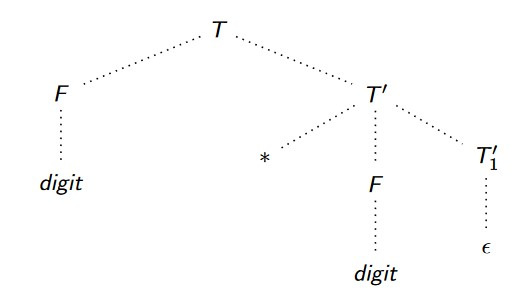
\includegraphics[width=.5\textwidth]{second-ex-parse-tree-part.jpg}
    \caption{Pezzo del parse tree di \(3*5\)}
    \label{fig:second-ex-parse-tree-part}
\end{figure}
Osserviamo come in questo caso abbiamo una digit che si trova nel sottoalbero sinistro della radice, mentre l'operatore \(*\) e l'altra digit si trovano nel sottoalbero destro della radice.
Come facciamo a fare in modo che \(T.val\) abbia valore \(15\)?

\noindent \emph{Chiediamo l'intervento degli attributi ereditati}

\noindent Questo è il caso in cui possiamo aiutarci con l'utilizzo di attributi ereditati, presentiamo in Fig.\ref{fig:second-ex-dependency-graph-part} come si possono utilizzare gli attributi ereditati; in blu abbiamo ancora una volta gli archi del grafo delle dipendenze e le etichette \(.i\) e \(.s\) rappresentano rispetivamente attributi ereditati e sintetizzati.
\begin{figure}[H]
    \centering
    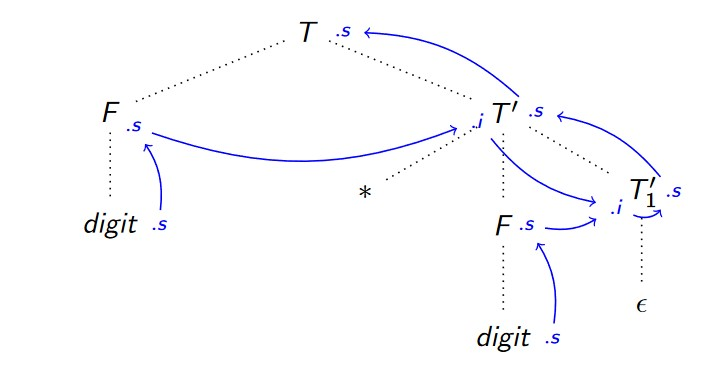
\includegraphics[width=.5\textwidth]{second-ex-dependency-graph-part.jpg}
    \caption{Pezzo del grafo delle dipendenze di \(3*5\)}
    \label{fig:second-ex-dependency-graph-part}
\end{figure}
Vediamo quindi come in questo caso sia necessario utilizzare gli attributi ereditati, che però aggiungono un livello di complessità.

Quando studiamo la regola per una produzione dobbiamo usare solo le informazioni che abbiamo a quel livello, in quella produzione, così viene affrontata la costruzione dell'SDD.

Andiamo ora a vedere nello specifico come viene affrontata la questione delle dipendenze quando si generano le regole per questo determinato SDD.
La prima cosa da notare è che quando il valore di \(T'\) viene copiato in \(T\) contiene già il valore della moltiplicazione.
In questo caso la regola che andiamo ad associare alla produzione rappresentata è
\begin{align*}
    T &\to FT' & & &\{T'.i = F.s; \; T.s = T'.s\}
\end{align*}
ovvero passiamo a \(T'\) come valore ereditato \(F.s\) ed assegnamo a \(T\) come valore sintetizzato \(T'.s\), il che viene rappresentata graficamente così:
\begin{figure}[H]
    \centering
    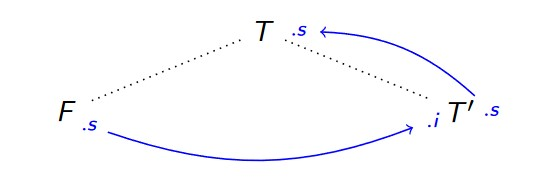
\includegraphics[width=.5\textwidth]{second-ex-dependency-graph-part-1.jpg}
    % \label{fig:second-ex-dependency-graph-part-1}
\end{figure}
Se andiamo invece ad osservare come viene generato il valore di \(T'\) vediamo dal pezzo di parse tree annotato in Fig.\ref{fig:second-ex-dependency-graph-part} che in pirmis ereditiamo un elemento dal fratello di sinistra, poi sappiamo che lo moltiplichiamo per il valore che ci è dato da \(F.s\) per ottenere il valore di \(T'_1\), che poi passeremo a \(T'\).

La regola per questa produzione è quindi
\begin{align*}
    T' &\to *FT_1' & & &\{T_1'.i = T'.i * F.s; \; T'.s = T_1'.s\}
\end{align*}
che si può rappresentare graficamente così:
\begin{figure}[H]
    \centering
    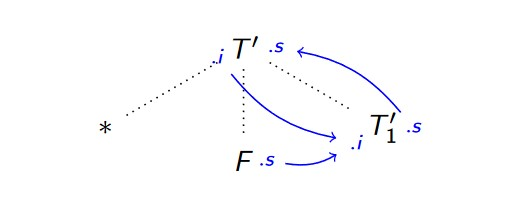
\includegraphics[width=.5\textwidth]{second-ex-dependency-graph-part-2.jpg}
    % \label{fig:second-ex-dependency-graph-part-1}
\end{figure}
Ora che abbiamo studiato i due punti critici dell'SDD per questa grammatica riportiamo l'SDD nella sua completezza.
\begin{align*}
    &V  \to E & &\{V.s = E.s\} \\
    &E  \to TE' & &\{E.s = E'.s; \; E'.i = T.s\} \\
    &E' \to +TE_1' & &\{E'.s = E_1'.s; \; E_1'.i = E'.i + T.s\} \\
    &E' \to \varepsilon & &\{E'.s = E'.i\} \\
    &T  \to FT' & &\{T.s = T'.s; \; T'.i = F.s\} \\
    &T' \to *FT_1' & &\{T'.s = T_1'.s; \; T_1'.i = T'.i * F.s\} \\
    &T' \to \varepsilon & &\{T'.s = T'.i\} \\
    &F  \to (E) & &\{F.s = E.s\} \\
    &F  \to digit & &\{F.s = digit.lexval\}
\end{align*}

\subsection{Traduzione durante il parsing}

Il nostro obiettivo è considerare la traduzione direttamente durante la fase di parsing per poter ottimizzare le attività della compilazione. Questo ci permette di evitare una prima elaborazione sintattica per ottenere il parse tree e la seconda, semantica, per valutare gli attributi.

Il caso più semplice in cui queste due elaborazioni possono essere eseguite in modo congiunto lo si ha considerando una grammatica adatta al parsing bottom-up a cui possiamo applicare l'algoritmo di shift/reduce (i.e. SLR(1), LR(1), LALR(1)) e l'SDD è S-attribuito (i.e. gli unici attributi presenti sono sintetizzati). Come mai?

L'algoritmo di shift/reduce si può eseguire con complessità lineare e necessità di due pile AA: una per mantenere gli stati (stSt) mentre l'altra per la catena dei simboli per poter conservare la derivazione parziale (sySt). L'idea è quella che insieme a queste due pile possiamo mantenerne una terza, che chiameremo \textbf{semSt}, dove conserveremo gli attributi (e.g. nel caso di una grammatica di espressioni aritmetiche degli interi).

\subsubsection{Esempio Algoritmo shift/reduce con semSt}

Per poter fornire un'idea di come utilizzare questa pila vediamo un esempio per cui è possibile valorizzare identificatori ed espressioni nel momento in cui si hanno a disposizione tutte le informazioni sugli attributi dei simboli del body. 

Consideriamo la seguente grammatica per definire le espressioni aritmetiche:
\begin{align*}
    V &\to E \\
    E &\to E + T \mid T \\
    T &\to T * F \mid F \\
    F &\to (E) \mid digit
\end{align*}

Il nostro obiettivo è quello di svolgere la traduzione durante il parsing ma per poter fare ciò abbiamo anche bisogno delle regole associate ad ogni produzione della grammatica

\begin{align*}
    V &\to E &\{print(E.val)\} \\
    E &\to E_1 + T &\{E.val = E_1.val + T.val\} \\
    E &\to T &\{E.val = T.val\} \\
    T &\to T_1 * F &\{T.val = T_1.val * F.val\} \\
    T &\to F &\{T.val = F.val\} \\
    F &\to (E) &\{F.val = E.val\} \\
    F &\to digit &\{F.val = digit.lexval\}
\end{align*}

Come abbiamo potuto osservare nei capitoli precedenti, l'algoritmo shift/reduce necessita della tabella di parsing per operare. La cortesia di poter osservare che tipo di operazioni venissero eseguite purtroppo non è stata concessa a quei poveri disgraziati che erano a lezione ma, per poter comprendere appieno l'esercizio, ci sentiamo in dovere di fornire, a chiunque stia leggendo, l'automa caratteristico e la relativa tabella di parsing LALR(1).

\begin{figure}[H]
    \centering
    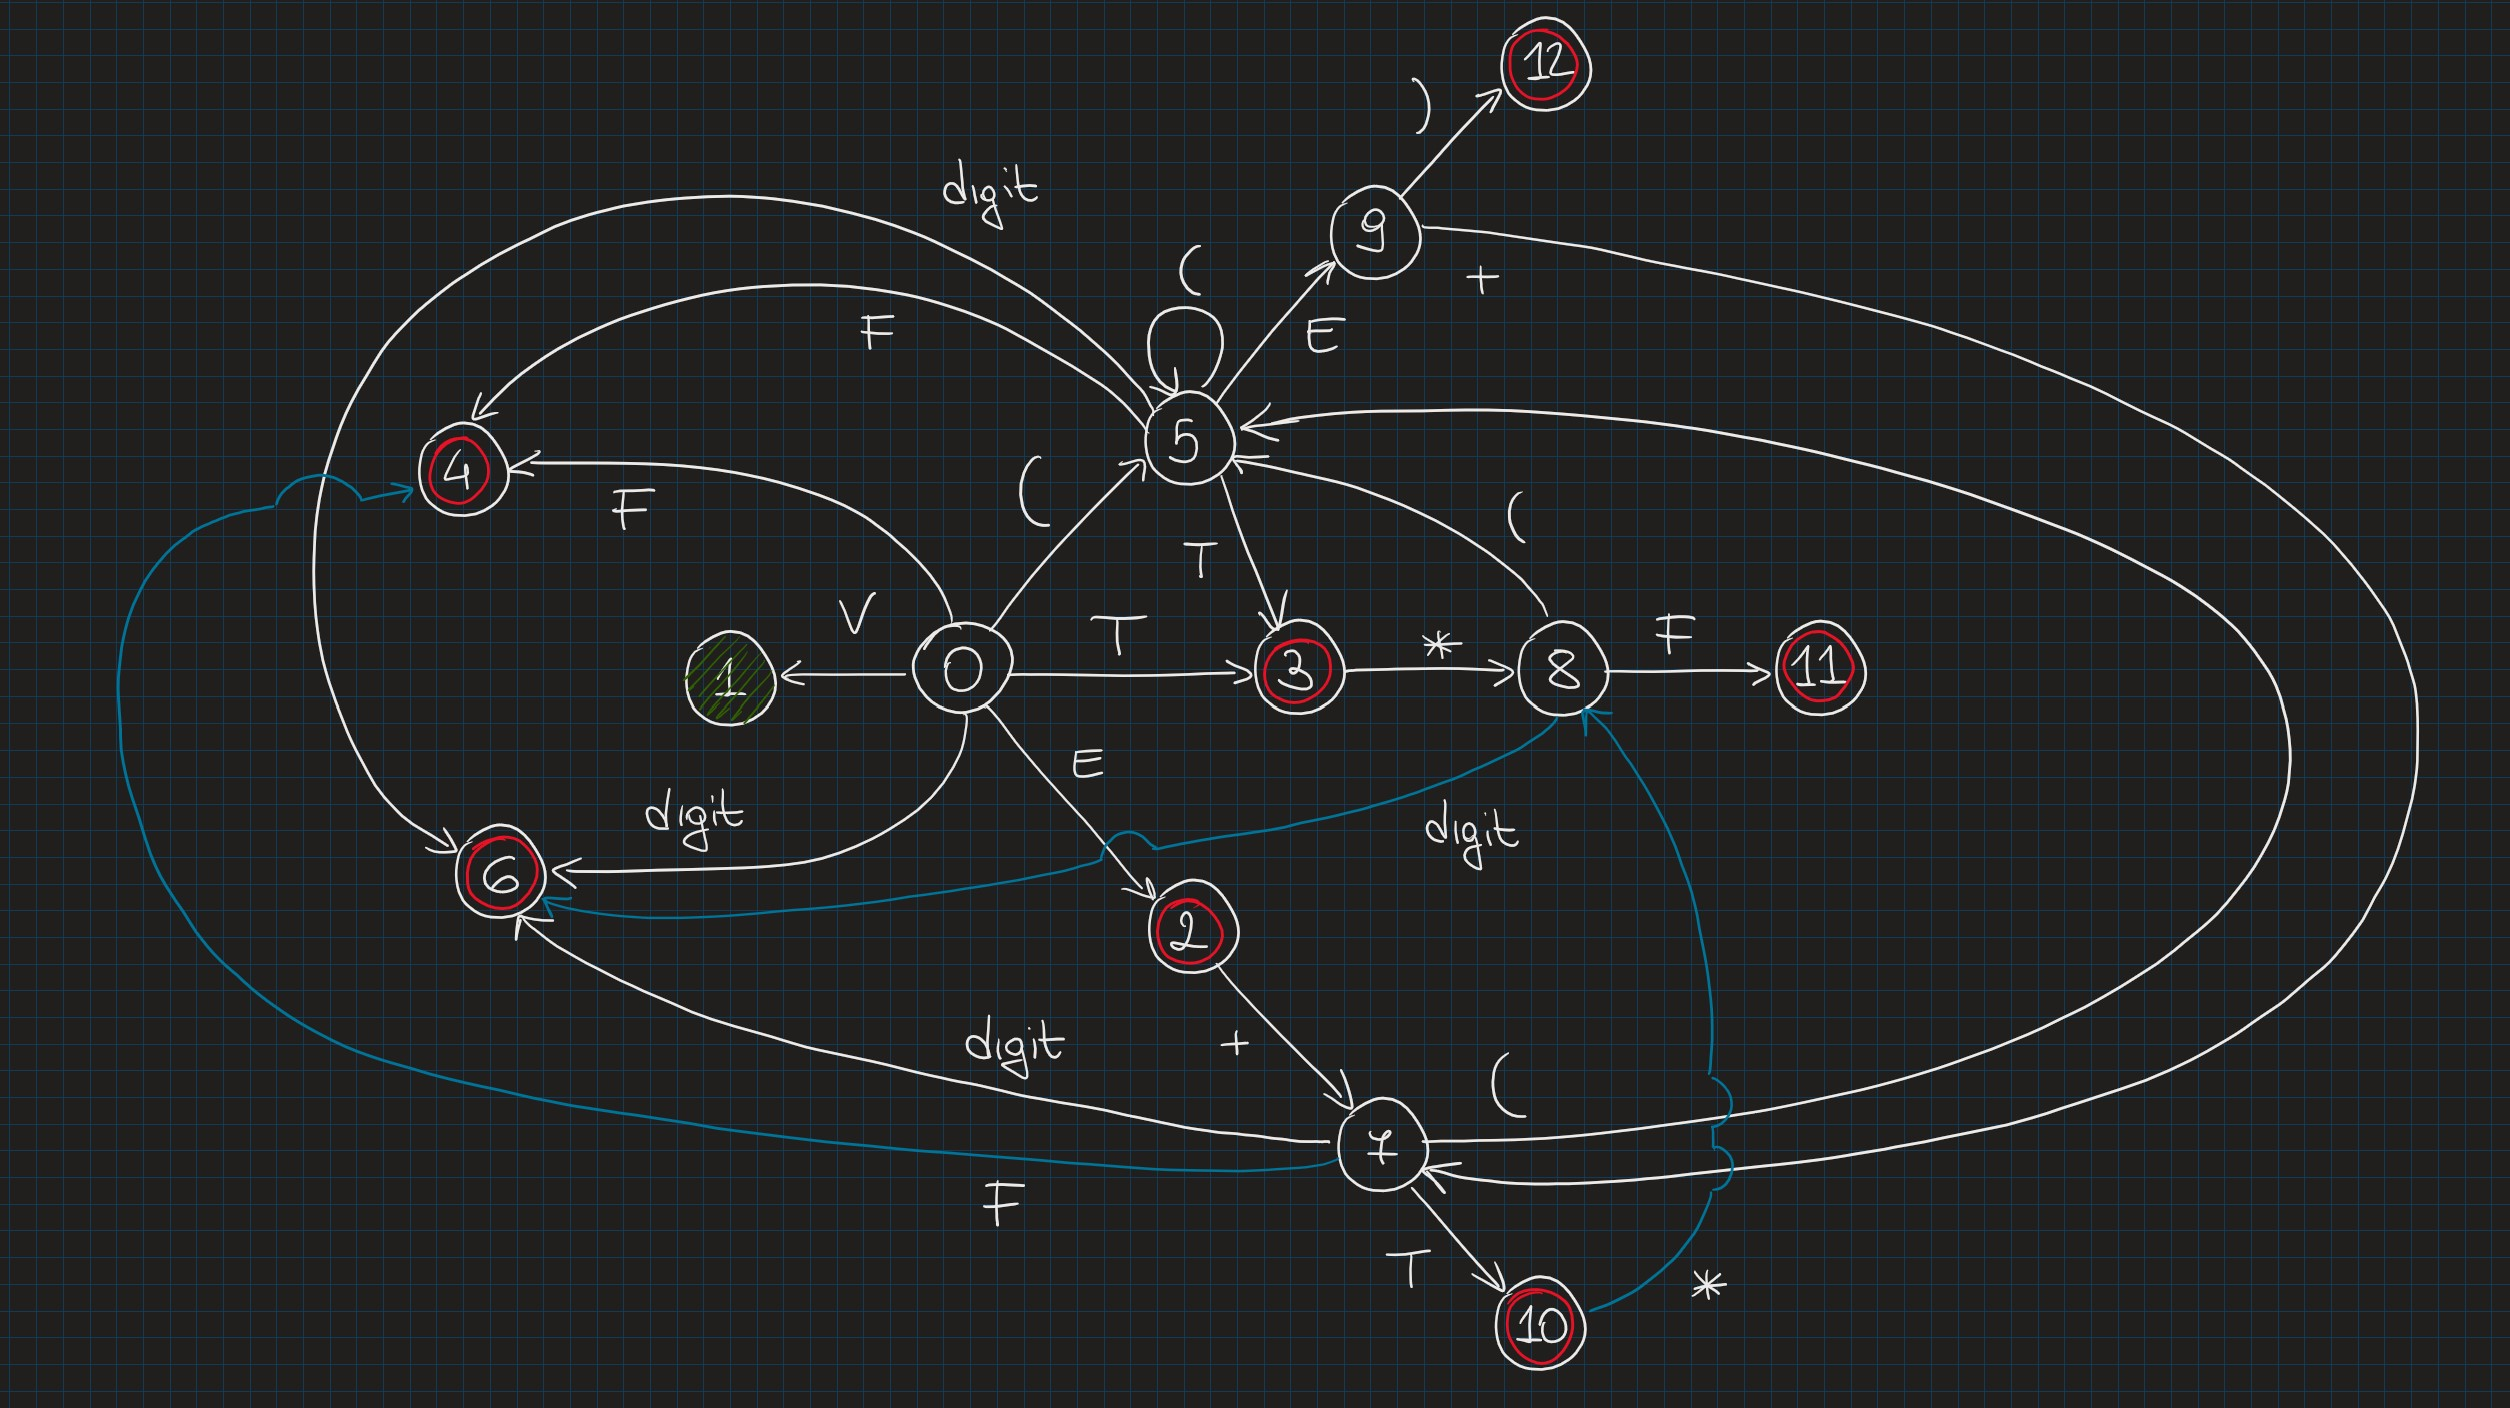
\includegraphics[width=1\textwidth]{lalr-automata.jpg}
\end{figure}

\begin{table}[H]
    \centering
    \subimport{assets/tables/}{lalr-parsing-table.tex}
    \caption{Tabella di parsing LALR(1) Espressioni Aritmetiche}
    \label{tab:lalr-parsing-table}
\end{table}

dove

\begin{itemize}
    \item[r1:] \(V \to E\) 
    \item[r2:] \(E \to E + T\)
    \item[r3:] \(E \to T\)
    \item[r4:] \(T \to T * F\)
    \item[r5:] \(T \to F\)
    \item[r6:] \(F \to (E)\)
    \item[r7:] \(F \to digit\)
\end{itemize}

Eseguiamo l'algoritmo shift/reduce dato in input \(w = digit + digit\$\) per la grammatica LALR(1) descritta poco sopra. Visto che vogliamo eseguire la traduzione degli attributi durante il parsing supponiamo che il primo abbia valore lessicale pari a 3 (i.e. \(digit.lexval = 3\)) mentre il secondo pari a 4; per questo motivo per poter mantenere traccia degli attributi faremo uso della pila \textbf{semSt} (semantic stack). 

Come sempre iniziamo partendo dallo stato 0 con la seguente situazione iniziale:

\begin{align*}
    w &= digit + digit\$ \\
    stSt &= 0 \\
    symSt &= \\     
    semSt &= \\
\end{align*}

Il primo simbolo che leggiamo dall'input buffer è \(digit\) quindi, come è possibile osservare sia dall'automa caratteristico che dalla parsing table, dobbiamo eseguire un'operazione di \texttt{shift} 6. Oltre che valorizzare le pile come durante un normale esecuzione dell'algoritmo eseguiamo \texttt{push} \(digit.lexval\) per poter inserire 3 sulla cima di \(semSt\) a seguito dell'operazione di shift.

\begin{align*}
    w &= \underline{digit} + digit\$ \\
    stSt &= 0\; 6 \\
    symSt &= digit \\     
    semSt &= 3 &\texttt{push}\;digit.lexval \\
\end{align*}

A questo punto il simbolo letto dall'input buffer è \(+\) e, visto che ci troviamo nello stato 6, abbiamo la possibilità di eseguire \texttt{reduce} \(F \to digit\): a seguito di un'operazione di riduzione dobbiamo anche eseguire il codice associato (i.e. la regola) con la produzione \(F \to digit\) (i.e. \(\{F.val = digit.lexval\}\)). In questo caso ciò si traduce in 

\begin{align*}
    w &= \underline{digit} + digit\$ \\
    stSt &= 0\; 4 \\
    symSt &= F &\texttt{reduce}\; F \to digit \\     
    semSt &= 3 &\texttt{pop}\;digit.lexval;\; \texttt{push}\;F.val = digit.lexval\\
\end{align*}

Nello stato 4 abbiamo nuovamente la possibilità di eseguire \texttt{reduce} \(T \to F\) leggendo dall'input buffer un \(+\): in questo caso la regola associata con la produzione è \(\{T.val = F.val\}\) per cui il procedimento sarà simile a quello precedente

\begin{align*}
    w &= \underline{digit} + digit\$ \\
    stSt &= 0\; 3 \\
    symSt &= T &\texttt{reduce}\; T \to F \\     
    semSt &= 3 &\texttt{pop}\;F.val;\; \texttt{push}\;T.val = F.val\\
\end{align*}

Il processo è analogo per lo stato 3 in cui eseguiremo una \texttt{reduce} \(E \to T\) e applicheremo la regola associata \(\{E.val = T.val\}\)

\begin{align*}
    w &= \underline{digit} + digit\$ \\
    stSt &= 0\; 2 \\
    symSt &= E &\texttt{reduce}\; E \to T \\     
    semSt &= 3 &\texttt{pop}\;T.val;\; \texttt{push}\;E.val = T.val \\
\end{align*}

Giunti finalmente nello stato 2 possiamo eseguire \texttt{shift} 7 che ci porta a consumare il simbolo \(+\) dall'input buffer. Visto che abbiamo eseguito uno shift dovremmo caricare il simbolo \(+\) sulla pila \(semSt\) ma ciò creerebbe un'inconsistenza in quanto, tecnicamente, dovrebbe contenere solamente solo dei numeri interi: per poter superare questa problematica carichiamo lo 0 come dummy in modo da mantenere l'allineamento con la pila dei simboli. 

\begin{align*}
    w &= \underline{digit \;+}\; digit\$ \\
    stSt &= 0\; 2\; 7 \\
    symSt &= E\; + \\     
    semSt &= 3\; 0 &\texttt{push}\;dummy\\
\end{align*}

Dallo stato 7 possiamo eseguire \texttt{shift} 6 leggendo dall'input buffer \(digit\): a questo punto possiamo caricare anche il valore del secondo digit sulla pila semantica. 

\begin{align*}
    w &= \underline{digit + digit}\$ \\
    stSt &= 0\; 2\; 7\; 6 \\
    symSt &= E + digit \\     
    semSt &= 3\; 0\; 4 &\texttt{push}\;digit.lexval\\
\end{align*}

Il processo a questo risulta essere analogo a quello fatto precedentemente per il primo \(digit\) quindi ci riserviamo la possibilità di non spiegare così nel dettaglio i prossimi passaggi 

\begin{align*}
    w &= \underline{digit + digit}\$ \\
    stSt &= 0\; 2\; 7\; 4 \\
    symSt &= E + F &\texttt{reduce}\; F \to digit\\     
    semSt &= 3\; 0\; 4 &\texttt{pop}\;digit.lexval;\; \texttt{push}\;F.val = digit.lexval\\
\end{align*}

\begin{align*}
    w &= \underline{digit + digit}\$ \\
    stSt &= 0\; 2\; 7\; 10 \\
    symSt &= E + T &\texttt{reduce}\; T \to F\\     
    semSt &= 3\; 0\; 4 &\texttt{pop}\;F.val;\; \texttt{push}\;T.val = F.val\\
\end{align*}

Nello stato 10 eseguiamo la \texttt{reduce} \(E \to E + T\) leggendo dall'input buffer \$. tale produzione è associata alla regola \(\{E.val = E_1.val + T.val\}\) che ci permette tra le varie cose di eseguire la somma e di rimuovere il dummy dal \(semSt\).

\begin{align*}
    w &= \underline{digit + digit}\$ \\
    stSt &= 0\; 2 \\
    symSt &= E &\texttt{reduce}\; E \to E + T\\     
    semSt &= 7 &\texttt{pop}\;T.val;\; \texttt{pop}\;dummy;\; \texttt{pop}\;E_1.val;\\ 
    && \texttt{push}\;E = E_1.val + T.val\\
\end{align*}

Dallo stato 2 possiamo eseguire questa volta \texttt{reduce} \(V \to E\) in quanto il simbolo che leggiamo dall'input buffer è \$: come sempre associamo a tale produzione la relativa regola (i.e. \(\{print(E.val)\}\)).

\begin{align*}
    w &= \underline{digit + digit}\$ \\
    stSt &= 0\; 1 \\
    symSt &= V &\texttt{reduce}\; V \to E;\; Acc \\     
    semSt &= 7 &\texttt{pop}\;E.val;\; print(E.val)\\
\end{align*}

Questo tipo di approccio è sempre possibile nel caso in cui l'SDD sia S-attribuito: essendo che siamo in grado di calcolare il valore degli attributi del padre di un sottoalbero solamente sulla base degli attributi dei suoi figli, il modo più facile di implementare l'algoritmo è eseguire le azioni nel momento in cui viene effettuata la riduzione (i.e. il momento in cui conosciamo tutti i valori dei figli). 

Avendo la possibilità di fare un po' più di pre-processing si riesce comunque in bottom-up ad eseguire tale procedura per SDD che sono L-attribuiti ma naturalmente aumenta la complessità. 

\subsection{Tradurre Stringhe in Numeri}

Analizziamo ora delle grammatiche che permettono di tradurre stringhe in numeri: l'idea è che data una certa stringa vogliamo ottenere il loro valore decimale. 

Possiamo pensare di scrivere una grammatica che genera il linguaggio delle stringhe di digit e il relativo schema di traduzione. 

La prima grammatica su cui ragioneremo è

\begin{align*}
    S &\to Digits	&\{print(Digits.v)\} \\
    Digits &\to Digits_1 d	&\{Digits.v = Digits_1.v * 10 + d.lexval\} \\
    Digits &\to d	&\{Digits.v = d.lexval\}
\end{align*}

La grammatica che abbiamo di fronte è LALR(1) e l'SDD è S-attribuito: l'ultima affermazione è verificabile dal fatto che il valore del padre dei sottolaberi possibili è sempre e solamente dipendente da quello dei figli. In questo caso dunque è possibile eseguire le due elaborazioni in modo congiunto e quindi possiamo calcolare il tutto durante il parsing. 

Aggiungiamo una variazione dell'esercizio: ora vogliamo tradurre stringhe di digit al loro valore interpretato in decimale oppure in ottale.

Una possibile grammatica che genera il linguaggio descritto è questa:

\begin{align*}
    S &\to Num \\
    Num &\to o \textrm{ } Digits \mid Digits \\
    Digits &\to Digits \textrm{ } d \mid d
\end{align*}

Quando ci troviamo nel caso di una stringa con il simbolo \(o\) davanti intendiamo che vogliamo ottenere il valore ottale della sequenza di digit. 

La grammatica anche in questo caso è LALR(1) però abbiamo un problema: non è possibile sintetizzare le informazioni nello stesso modo di prima in quanto queste non sono disponibili nel momento in cui ci servono. Ragionando infatti sulla derivazione \(S \Rightarrow Num \Rightarrow o Digits\) ci si rende conto del fatto che il simbolo \(o\) si trova nel sottoalbero sinistro dell'albero mentre i \(Digits\) in quello destro: questo vuol dire che di fatto non siamo in grado di calcolare il valore fino a quando non raggiungiamo la cima dell'albero e quindi ciò significa che non ci troviamo di fronte a un SDD S-attribuito (il valore del sottoalbero di destra dipende infatti dal valore dei fratelli e non solamente da quello dei figli).

Per poter raggiungere i nostri obbiettivi a livello di efficienza dobbiamo riprovare modificando la grammatica in modo che ci consenta di svolgere entrambe le operazioni contemporaneamente.

Per poter ottenere un risultato migliore potremmo inserire due nuovi non terminali in modo da poterci aiutare con le regole in un secondo momento: consideriamo infatti di modificare la grammatica nel modo seguente

\begin{align*}
    S &\to Num \\
    Num &\to O \textrm{ } Digits \mid D \textrm{ } Digits \\
    O &\to o \\ 
    D &\to \varepsilon \\
    Digits &\to Digits \textrm{ } d \mid d
\end{align*}

Di per sé non sembra essere cambiato molto ma in realtà in questo caso abbiamo la possibilità di inserire delle regole dove possiamo valorizzare delle variabili globali in modo da stabilire la base:

\begin{align*}
    S &\to Num &\{print(Num.v)\}\\
    Num &\to O \textrm{ } Digits &\{Num.v = Digits.v\}\\
    Num &\to D \textrm{ } Digits &\{Num.v = Digits.v\}\\
    O &\to o &\{base = 8\}\\ 
    D &\to \varepsilon &\{base = 10\}\\
    Digits &\to Digits_1 \textrm{ } d &\{Digits.v = Digits_1.v * base + d.lexval\}\\
    Digits &\to d &\{Digits.v = d.lexval\}
\end{align*}

Stabilendo separatamente la base mediante le regole abbiamo dunque la possibilità di poter svolgere tutti i calcoli necessari senza rinunciare all'efficienza. 

\section{Alberi di Sintassi Astratta}
\subsection{Introduzione}
Arriviamo finalmente a parlare degli alberi di sintassi astratta (Abstract Syntax Trees) che altro non sono che una rappresentazione compatta degli alberi di derivazione.

Un albero di sintassi astratta si può ottenere dal rispettivo albero di derivazione di una parola tramite dei passi di semplificazione, per avere chiaro a cosa ci riferiamo facciamo subito un esempio.
Sia data la grammatica
\begin{align*}
    E &\to E+T \mid T \\
    T &\to T*F \mid F \\
    F &\to (E) \mid id \\
\end{align*}
Se vogliamo fare il parsing della parola \(digit+digit\) otteniamo i seguenti alberi di parsing e di sintassi astratta.
\begin{figure}[H]
    \centering
    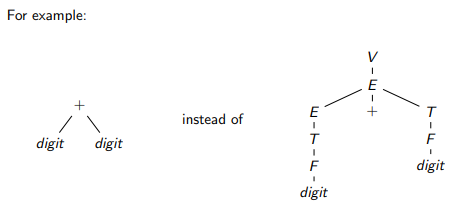
\includegraphics[width=.8\textwidth]{ast-first-example.png}
    \caption{Due alberi per la parola \(digit+digit\): sulla sinistra albero di sintassi astratta, sulla destra albero di derivazione}
    \label{fig:ast-first-example}
\end{figure}
Si noti come l'albero della sintassi astratta a sinistra sia molto più compatto.

\paragraph{Memorizzazione degli AST} Di fatto questa struttura va a creare in memoiria un albero in cui ogni nodo rappresenta un passaggio intermedio del processo descritto dalla parola che stiamo analizzando. L'AST ottenuto dalla semplificazione dell'albero di derivazione viene quindi salvato nodo per nodo nel seguente modo:
\begin{itemize}
    \item le foglie vengono salvate come link a record nella tabella dei simboli: viene creata una foglia per ogni identificatore ed ogni valore diretto (es.: valore numerico) presente nella parola che stiamo parsando;
    \item i nodi intermedi dell'albero costituiscono la struttura topologica dell'albero e rappresentano tutte le operazioni compiute tra variabili o valori diretti (quindi tutte le operazioni tra altri nodi).
\end{itemize}

\subsection{Creazione di un AST}
L'AST si può creare semplicemente dopo aver ottenuto l'albero di derivazione tramite delle operazoni di compattazione, tuttavia il nostro obiettivo è quello di calcolare l'AST direttamente durante la fase di parsing, ovvero contemporaneamente all'analisi sintattica.
Per fare questo dobbiamo immaginare di avere a disposizione due funzioni:
\begin{itemize}
    \item \texttt{newLeaf(label, val)} che va a salvare un nodo foglia con due campi: l'etichetta ed il valore;
    \item \texttt{newNode(label, c1, ..., ck)} che crea un nodo con \(k\) figli, l'etichetta (che indica l'operazione rappresentata dal nodo) è \texttt{label} mentre \texttt{c1, ..., ck} sono i riferimenti ai nodi figli;
\end{itemize}
Applicando queste due funzioni all'esempio precedente (Fig.\ref{fig:ast-first-example}) avremo l'operazione \(+\) rappresentata da un nodo che avrà come etichetta \(+\) e come figli i due nodi \(digit\).
I nodi \(digit\) saranno nodi foglia con identificatore e valore relativo (il valore sarà quello che ci viene ritornato dall'analisi lessicale, quindi lo possiamo ricavare con \(digit.lexval\)).\\

\paragraph{Funzioni di attribuzione} Per creare l'albero di sintssi astratta durante la fase di parsing dobbiamo definire delle regole semantiche (dette anche funzioni di attribuzione o azioni semantiche) che, ogni volta che incontriamo una riduzione, ci indichino quando e come istanziare un nodo per l'AST durante il parsing.

\noindent Vediamo un esempio: data la grammatica LALR per operazioni algebriche di somma e sottrazione 
\begin{align}
    \label{gr:LALR-plus-minus-grammar}
    E &\to E+T \mid E-T \mid T \\  
    T &\to (E) \mid id \mid num \notag \nonumber
\end{align}
abbiamo che le regole (le funzioni di attribuzione) per la creazione dell'AST durante il parsing sono le seguenti
\begin{align}
    \label{SDD:LALR-grammar}
    E &\to E_1+T & & \{E.node = newNode(\textrm{'}+\textrm{'}, E_1.node, T.node)\} \\
    E &\to E_1-T & & \{E.node = newNode(\textrm{'}-\textrm{'}, E_1.node, T.node)\} \notag \nonumber \\
    E &\to T & & \{E.node = T.node\} \notag \nonumber \\
    T &\to (E) & & \{T.node = E.node\} \notag \nonumber \\
    T &\to id & & \{T.node = newLeaf(id, id.entry)\} \notag \nonumber \\
    T &\to num & & \{T.node = newLeaf(num, num.lexval)\} \notag \nonumber
\end{align}
Si ricorda che i pedici numerici usati in alcune produzioni sono usati solo per differenziare il body dal driver, non hanno nessuna valenza semantica, di fatto \(E_1\) ed \(E\) sono lo stesso non-terminale.

Analizziamo velocemente le regole più significative:
\begin{itemize}
    \item \(newLeaf(num, num.lexval)\) va a prendere il valore di num che ci è dato dall'analisi lessicale; 
    \item in modo simile \(newLeaf(id, id.entry)\) va a creare un nodo foglia in cui abbiamo come etichetta l'identificatore mentre il valore del nodo si troverà all'interno della tabella dei simboli compilata in fase di analisi lessicale.
\end{itemize}

Per le altre regole il significato, abbastanza intuitivo, è quello della creazione di un nodo intermedio che mantiene come informazioni l'etichetta dell'operazione da compiere e i riferimenti ai nodi degli operandi necessari.

\subsubsection{Esempio di creazione di un AST}
Ora che abbiamo le regole da applicare per costruire un albero di sintassi astratta, andiamo a costruirne uno per la parola \(id-num+id\) derivata dalla grammatica appena vista (\ref{gr:LALR-plus-minus-grammar}), immaginando che la parola \(id-num+id\) sia arrivata dall'analisi lessicale di \(a-4+c\).

\noindent Innanzitutto dobbiamo arrivare alla fase del parsing, quindi ci dobbiamo procurare la tabella di parsing.

\noindent O almeno questo ci saremmo aspettati da un esercizio normale, ma invece no! La nostra guida spirituale a questo punto ci fa notare che abbiamo imparato a fare le tabelle di parsing per imparare a non farle più: dato che ci serve solo l'ordine delle produzioni utilizzate per ottenere la parola che stiamo analizzando possiamo barare e fare la derivazione a mente.

Quindi, tornando a noi e saltando qualche passaggio (che forse verrà inserito in seguito, dipende da quanto verranno pagati gli scrittori della dispensa), la sequenza di riduzioni che si ottiene dal parsing della parola \(id-num+id\) è la seguente:
\begin{align*}
    T &\to id \\
    E &\to T \\
    T &\to num \\
    E &\to E-T \\
    T &\to id \\
    E &\to E+T
\end{align*}
Si invita il lettore a fermarsi un attimo e rileggere queste produzioni per convincersi che siano esattamente le riduzioni che si ottengono dal parsing bottom-up della parola data; si faccia attenzione all'ordine in cui si incontrano le riduzioni, questo è proprio l'ordine che ci si aspetta dalla procedura bottom-up, ovvero l'ordine inverso della procedura che dallo start symbol ci porta alla parola desiderata.

Vediamo ora come viene creato in memoria l'Abstract Syntax Tree mentre stiamo svolgendo il parsing della stringa.
Ogni volta che incontriamo una riduzione andiamo ad aggiungere un nodo all'AST che stiamo creando. Quale forma avrà questo nodo ci è dato dalle funzioni di attribuzione dei nodi dell'AST.
Osserviamo quindi quale forma viene ad ottenere l'abero di sintassi astratta della nostra parola \(id-num+id\) mentre incontriamo le riduzioni passo dopo passo.
\begin{enumerate}
    \item La prima riduzone che incontriamo è \(T \to id\), che ha come funzione di attribuzione \(\{T.node = newLeaf(id, id.entry)\}\); la rappresentazione grafica di quello che si ottiene in questo caso è la seguente:
    \begin{figure}[H]
        \centering
        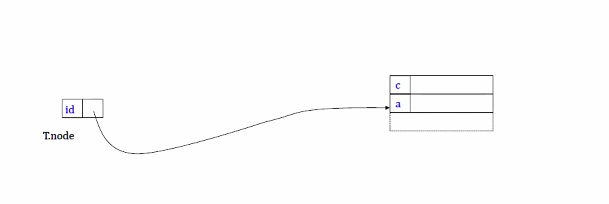
\includegraphics[width=.6\textwidth]{ex-ast-creation-1.png}
        \caption{Creaizone del nodo foglia per l'identificatore che referenzia la variabile \(a\)}
    \end{figure}
    \item La seconda riduzione che incontriamo, \(E \to T\), ci porta ad un semplice passaggio di rinominazione di un nodo dell'AST, in quanto la sua azione semantica è \(\{E.node = T.node\}\).
    \begin{figure}[H]
        \centering
        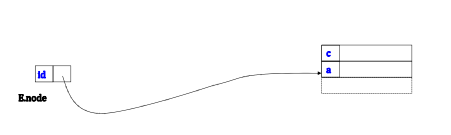
\includegraphics[width=.6\textwidth]{ex-ast-creation-2.png}
        \caption{Rinominazione del \(T.node\) in \(E.node\)}
    \end{figure} 
    \item Il terzo passo ci porta ad usare la riduzione \(T \to num\), con annessa funzione di attribuzione \(\{T.node = newLeaf(num, num.lexval)\}\), che crea una nuova foglia con valore numerico associato.
    \begin{figure}[H]
        \centering
        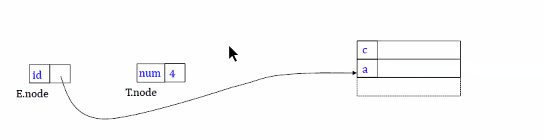
\includegraphics[width=.6\textwidth]{ex-ast-creation-3.png}
        \caption{Creazione di una nuova foglia con valore numerico associato}
    \end{figure} 
    \item La prossima riduzione che incontriamo è \(E \to E_1 - T\), con azione semantica \(\{E.node = newNode('-', E_1.node, T.node)\}\), che viene rappresentata graficamente creando un nuovo nodo intermedio per l'AST, la cui forma può essere osservata nella figura sottostante.
    \begin{figure}[H]
        \centering
        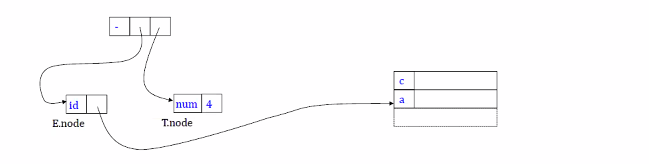
\includegraphics[width=.6\textwidth]{ex-ast-creation-4.png}
        \caption{Inserimento del nodo intermedio che rappresenta la sottrazione}
    \end{figure} 
    \item In seguito ci scontriamo di nuovo in una riduzione \(T \to id\), che ha come funzione di attribuzione \(\{T.node = newLeaf(id, id.entry)\}\), sappiamo già come funziona dal primo punto di questa lista. La rappresentazione grafica del nostro AST a questo stadio è la seguente:
    \begin{figure}[H]
        \centering
        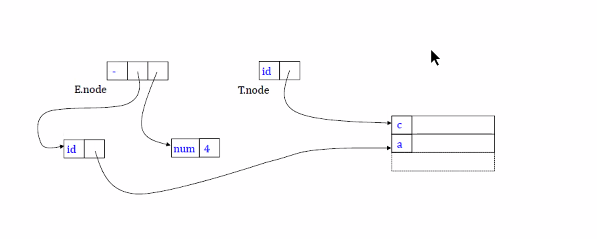
\includegraphics[width=.6\textwidth]{ex-ast-creation-5.png}
        \caption{Creazione di un nodo foglia per \(id\) associato a \(c\)}
    \end{figure} 
    \item Infine applichiamo la riduzione \(E \to E_1 + T\), che prevede l'azione semantica \(\{E.node = newNode ('+', E_1.node, T.node)\}\) e va a completare il nostro AST che possiamo finalmente osservare in tutta la sua bellezza:
    \begin{figure}[H]
        \centering
        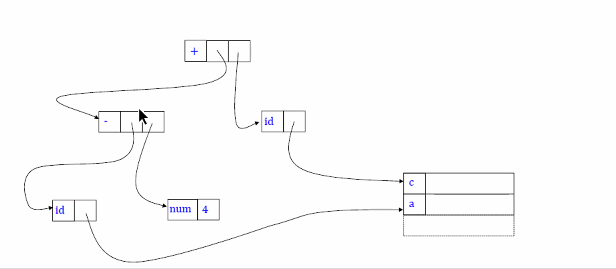
\includegraphics[width=.6\textwidth]{ex-ast-creation-6.png}
        \caption{Inserimento del nodo intermedio per la rappresentazione della somma}
    \end{figure} 
\end{enumerate}

\paragraph{Riassumendo} Il goal che ci siamo fissati all'inizio di questo esercizio era di costruire \emph{on the fly} l'albero di sintassi astratta durante la fase di parsing per la parola \(id-num+id\) derivata grammatica LALR per le espressioni aritmetiche (\ref{gr:LALR-plus-minus-grammar}).
Anche se abbiamo barato, utilizzando un parsing già fatto, è facile accorgersi che le funzioni di attribuzione che abbiamo usato ora le avremmo potute usare in contemporanea all'esecuzione del parsing, usandole direttamente ogni volta che avremmo incontrato una riduzione.

\noindent Per quanto riguarda le riduzioni con soli terminali nel body (che generano le foglie) abbiamo utilizzato questi attributi sintetizzati:
\begin{itemize}
    \item[\textbf{Id.entry}] per le variabili;
    \item[\textbf{Num.lexval}] per i valori numerici.
\end{itemize}
Mentre per le riduzioni con non-terminali nel body abbiamo utilizzato delle funzioni di attribuzione semantica che prevedono di inserire i seguenti attributi sintetizzati:
\begin{itemize}
    \item[\textbf{E-node}] per le riduzioni con driver E;
    \item[\textbf{T-node}] per le riduzioni con driver T.
\end{itemize}

Abbiamo visto quindi che si può ricavare l'AST mentre si esegue il nostro caro parsing bottom-up.
Ma non è sempre così, l'albero di sintassi astratta in questo caso è stato costruito su una grammatica LALR con un SDD con tutti attributi sintetizzati (vedi \ref{SDD:LALR-grammar}, non ci sono attributi ereditati), è questo che ci ha permesso di costruire l'AST mentre costruivamo l'albero di parsing.

Sottolineamo questo aspetto per dire che nel caso in cui abbiamo un SDD L-attribuito non è detto che si possa compiere la costruzione dell'AST mentre si fa il parsing. Per aver ragion di ciò presentiamo subito un esempio in cui compaiono appunto attributi ereditati.

\subsection{Esempio di creazione di un AST con attributi ereditati}
L'esercizio in questo caso ci richiede di calcolare gli attributi per definire le funzioni di attribuzione per le produzioni della grammatica così definita:
\begin{align}
    \label{SDD:ex-2-AST}
    E &\to TE' & & \{...\} \\ 
    E'&\to +TE_1' & & \{...\} \notag \nonumber \\ 
    E'&\to -TE_1' & & \{...\} \notag \nonumber \\ 
    E'&\to \varepsilon & & \{...\} \notag \nonumber \\ 
    T &\to (E) & & \{...\} \notag \nonumber \\ 
    T &\to id & & \{...\} \notag \nonumber \\ 
    T &\to num & & \{...\} \notag \nonumber
\end{align}
In questo caso dobbiamo chiamare in causa gli attributi ereditati, e la motivazione è presto detta.
Per visualizzare la situazione possiamo andare a rivedere l'SDD che abbiamo costruito per le operazioni \(+\) e \(*\) nella prima parte riguardo l'analisi semantica (Fig.\ref{fig:second-ex-parse-tree-part}, ma si può osservare tranquillamente la figura  qui sotto per rendersi conto).
In quel caso i valori sintetizzati in sottoalberi fratelli devono essere utilizzati da altri sottoalberi fratelli per ricavare il loro proprio valore, per esser chiari riportiamo qui la figura.
\begin{figure}[H]
    \centering
    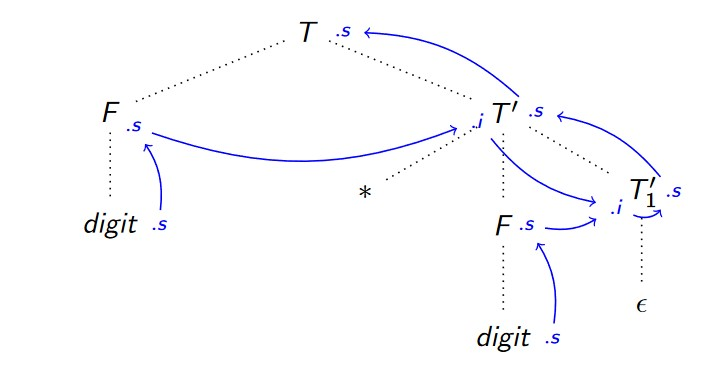
\includegraphics[width=.5\textwidth]{second-ex-dependency-graph-part.jpg}
    \caption{Pezzo del grafo delle dipendenze di \(3*5\)}
\end{figure}
Osservando quest'immagine è esemplice notare che per risolvere il valore di \(T'\) abbiamo bisogno dei valori nel sottoalbero di \(T'\) ma anche del valore di \(F\) che è fratello sinistro di \(T'\), quindi abbiamo bisogno di introdurre attributi ereditati.
Lo stesso avviene per la grammatica che stiamo considerando ora, quella per gli operatori \(+\) e \(-\) di cui dobbiamo completare l'SDD (\ref{SDD:ex-2-AST}).


%TODO bisogna mergiare queste due parti solo che non so che cosa è meglio tenere come introduzione
% Ti dirò che a me sembrano carini così

Il problema in questo caso specifico è che non possiamo sintetizzare tutte le informazioni che ci servono perchè, uno degli elementi necessari per ricavare il valore dell'espressione e per la formazione dell'abstract syntax tree, non è presente nello stesso sottoalbero nel quale troviamo l'operatore aritmetico e l'altro operando coinvolto nell'operazione. 

Utilizzando gli attributi ereditati non si riesce ad eseguire in maniera immediata tutte le operazioni durante il parsing della grammatica: un'opzione, come già citato più volte, potrebbe essere quella di agire sulla grammatica in modo che, durante un'esecuzione del parsing bottom-up, si possa ottenere lo stesso risultato di una grammatica S-attribuita. Senza soffermarci troppo sui dettagli, tale operazione passerebbe per l'aggiunta di marker e \(\varepsilon\)-transizioni in modo che gli attributi vengano sintetizzati e non ereditati.

In questo caso per poter trasportare le informazioni da un ramo dell'albero ad un altro è necessario utilizzare degli attributi ereditati: in modo simile a quanto fatto per calcolare il valore delle espressioni aritmetiche, in questo caso assegniamo dei riferimenti a dei nodi. 

Per poter capire al meglio che tipo di regole devono essere applicate è necessario partire da un parse tree: prendiamo dunque come esempio particolare la parola \(id - num\), ottenuta dall'analisi lessicale di \(a - 4\); senza troppa fatica dovremmo poterci accorgere che usando una derivazione di tipo leftmost i passi di derivazione sono

\begin{align*}
    E \Rightarrow TE' \Rightarrow idE' \Rightarrow id-TE' \Rightarrow id-numE' \Rightarrow id-num
\end{align*}

Il nostro \emph{parse tree} in questo particolare caso è così costruito

\begin{figure}[H]
	\centering
    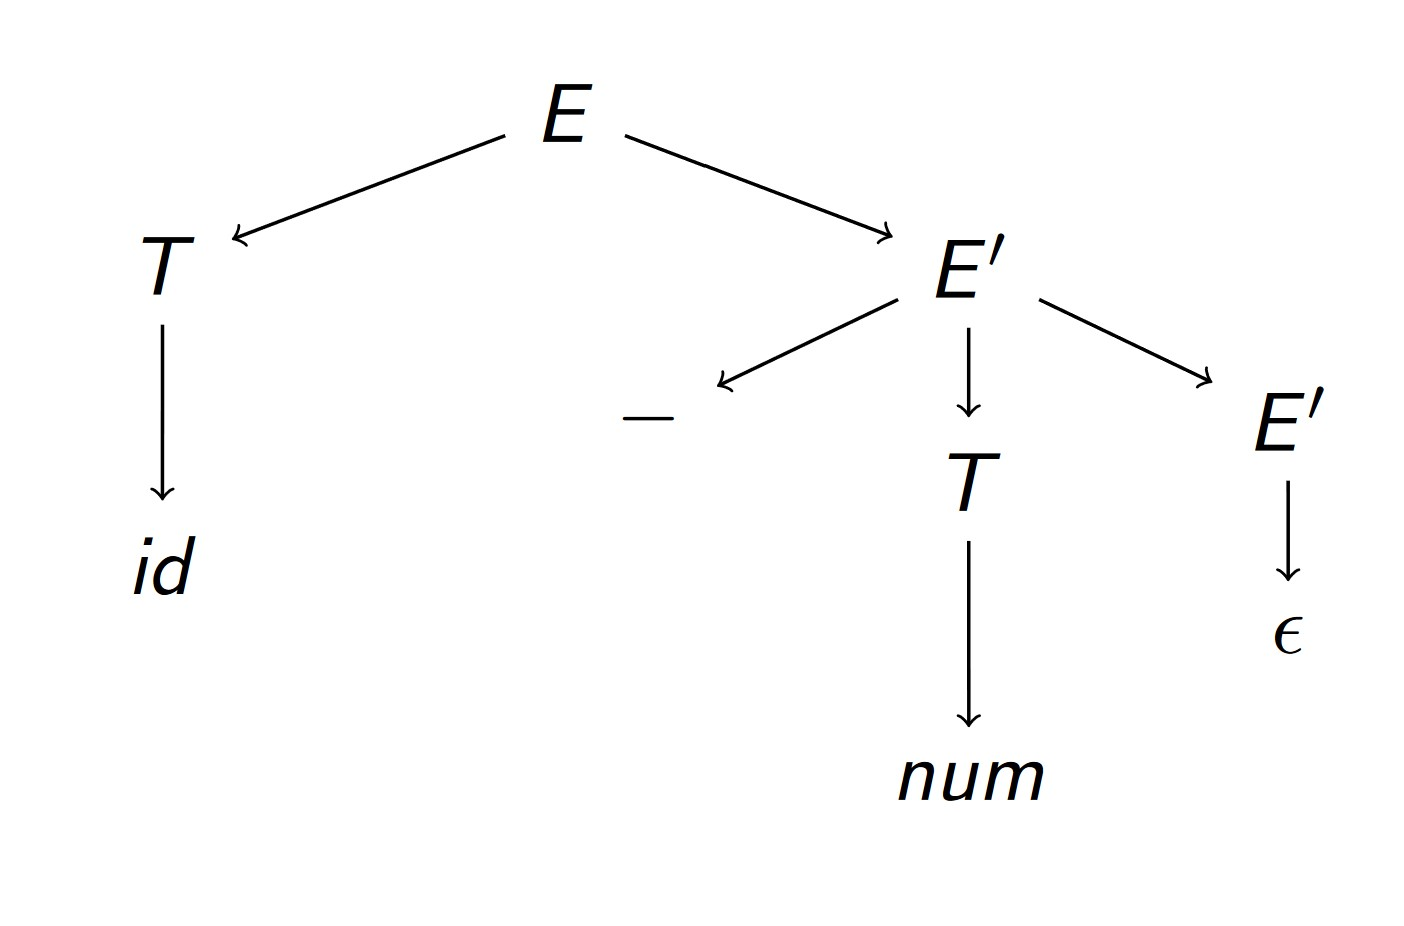
\includegraphics[width=.6\textwidth]{parse-tree-ae.jpg}
    \caption{parse tree attributi ereditati}
    \label{fig:parse-tree-ae}
\end{figure}

Dal parse tree possiamo osservare in modo più esplicito che il calcolo del sottoalbero destro (con radice in \(E'\)) necessita del sottoalbero sinistro (con radice in \(T\)) e quindi avremo bisogno degli attributi ereditati (quindi non potremo eseguire il parsing e la costruzione dell'abstract syntax tree contemporaneamente).

Facendo delle osservazioni di questo tipo siamo in grado di costruire la prossima struttura che ci servirà, cioè il \emph{dependency graph}: 

\begin{figure}[H]
	\centering
    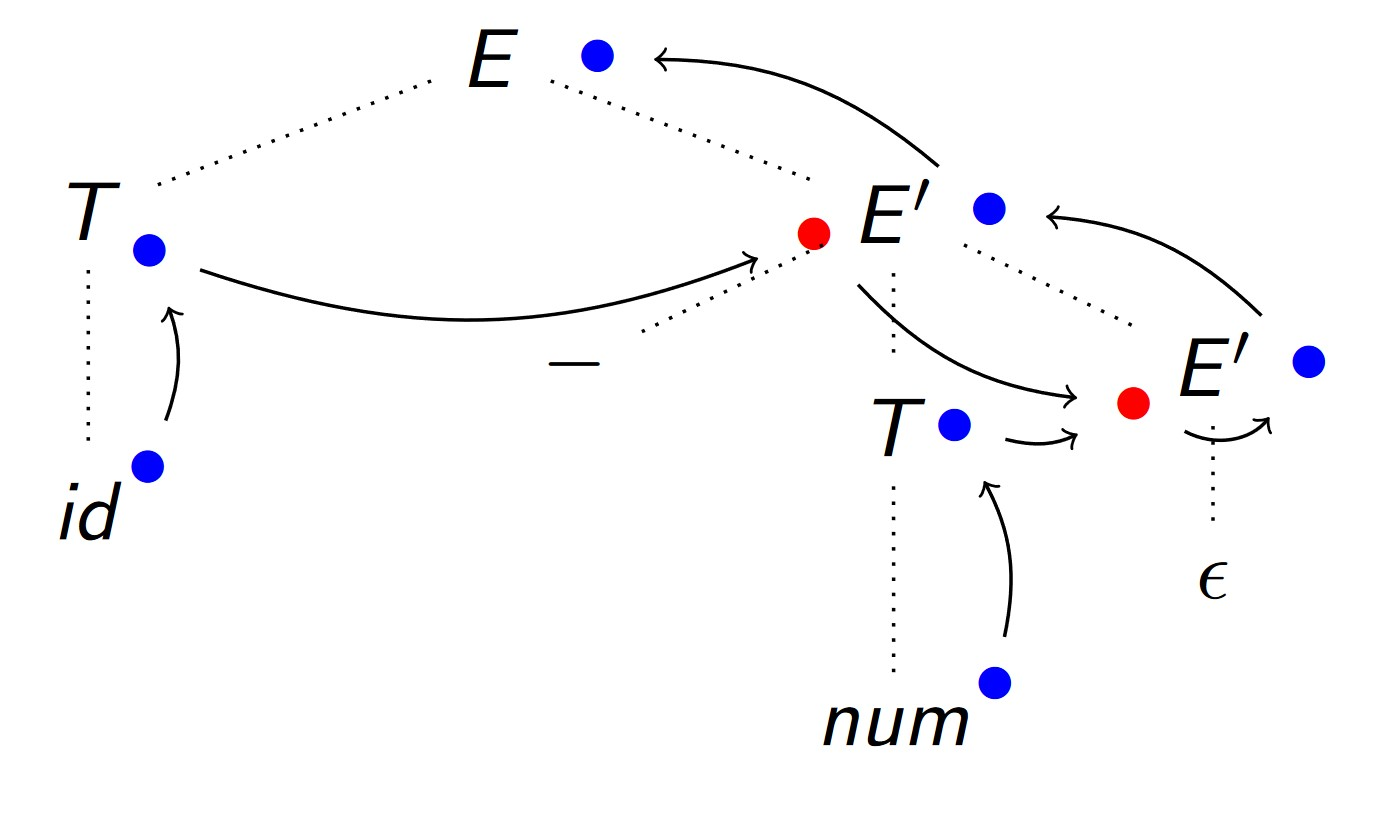
\includegraphics[width=.6\textwidth]{dependency-graph-ae.jpg}
    \caption{Dependency graph attributi ereditati}
    \label{fig:dependency-graph-ae}
\end{figure}

Può sembrare difficile ottenere questa struttura dal nostro parse tree, tuttavia i suoi archi rappresentano semplicemente le dipendenze tra gli attributi (i.e. quali sono necessari per poter effettuare una certa operazione); nella figura possiamo inoltre vedere quali fra gli attributi sono sintetizzati (in blu) e quali ereditati (in rosso). 

Per rendere più chiaro il grafo utilizziamo un esempio: il sottoalbero sinistro possiede un arco da \(id\) a \(T\) (coincidente con quello del parse tree) perché sottolineiamo che, una volta effettuata l'operazione di riduzione \(T \to id\), \(T\) mantenga un riferimento a \(id\); visto che \(id\) è contenuto nel sottoalbero di \(T\) (i.e. è uno dei suoi figli) tale attributo è sintetizzato. 

La situazione cambia se vogliamo esaminare l'arco esattamente successivo: l'arco da \(T\) ad \(E'\) infatti non coincide con nessun altro arco del parse tree e il suo scopo è quello di trasmettere i riferimenti di \(T\) al fratello \(E'\). Questa operazione viene fatta perchè, per poter calcolare in questo caso la differenza, è necessario che \(E'\) riceva le informazioni del fratello \(T\): dovremo dunque servirci di un attributo ereditato.

A questo punto dobbiamo definire le \textbf{funzioni di attribuzione} associate alle produzioni: tale operazione come sempre non è facile da eseguire ma vedremo di analizzarla passo per passo. 

Cominciamo inserendo le azioni semantiche delle produzioni finali della grammatica proposta: queste definiscono le foglie del nostro parse tree e dovranno occuparsi di generare gli elementi finali dell'sbstract syntax tree.

\begin{align*}
    T &\to id &\{T.node = newLeaf(id, id.entry)\} \\
    T &\to num &\{T.node = newLeaf(num, num.lexval)\}
\end{align*}

Queste produzioni ci permettono di creare due foglie:

\begin{itemize}
    \item una foglia con etichetta \(id\) e valore \(id.entry\) (i.e. quindi un riferimento alla sua entry nella symbol table per poter recuperare successivamente le informazioni);
    \item una seconda foglia con etichetta \(num\) e valore \(num.lexval\) (i.e. il valore ottenuto dall'analisi lessicale)
\end{itemize}

Come si può intuire, il nostro scopo con tali regole è fare in modo che in T.node siano memorizzate le informazioni della foglia che abbiamo creato in modo da poterle recuperare in seguito.

Come avevamo già potuto mostare in precedenza, il sottoalbero sinistro ha bisogno di passare le proprie informazioni al sottoalbero destro; visto che stiamo parlando di nodi fratelli non possiamo ottenere queste informazioni in altro modo se non ricorrendo agli attributi ereditati: ci servirà dunque una regola del tipo \(E'.i = T.node\).

Associamo dunque per il momento la regola descritta alla produzione corretta 

\begin{align*}
    E &\to TE' &\{E'.i = T.node\}
\end{align*}

Volendo chiarire subito alcuni possibili dubbi, sottolineo il fatto che questa non sarà l'unica regola che sarà associata a tale produzione (si è voluto optare per un aggiunta graduale) e che le produzioni a cui è stata aggiunta l'azione semantica sono quelle dove \(T\) ed \(E'\) compaiono nel body.

A questo punto possiamo passare alle produzioni che si occupano delle operazioni aritmetiche, nel nostro caso della produzione \(E' \to -TE'\): per via del nostro esempio potremmo limitarci semplicemente ad eseguire il risultato dell'espressione \(E'.i - T.node\) (ricordiamoci che precedentemente abbiamo fatto in modo che \(E'.i\) contenesse il valore del sottoalbero sinistro), tuttavia dobbiamo considerare anche i casi per cui vi potrebbero essere altre operazioni in seguito (e.g. id + id - num + id - ...). Per questo motivo facciamo in modo di passare ad \(E'\) il risultato di tale operazione in modo che possa utilizzarlo nel caso di produzioni successive: questo potrebbe essere visto come un esempio di ricorsione dove di fatto stiamo "mandando avanti" i risultati delle operazioni e dovremo in seguito capire qual è il nostro caso base. Aggiungiamo dunque una regola che fa al caso nostro 

\begin{align*}
    E' &\to -TE_{1}' &\{E_{1}'.i = newNode('-', E'.i, T.node)\}
\end{align*}

Grazie a questa azione semantica siamo in grado di generare un nodo con etichetta \(-\) e con un riferimento per ogni operando: il riferimento di questo nodo viene passato poi ad \(E_1'.i\), in questo modo riuscirà a svolgere le operazioni successive. 

Come abbiamo detto precedentemente, dovremo prima o poi interrompere tale ricorsione e quindi necessitiamo di un caso base: banalmente smetteremo di fare nuove chiamate nel momento in cui non avremo più operatori e quindi nel caso in cui utilizzeremo la produzione \(E' \to \varepsilon\). In questo momento dovremo riportare il risultato di tutta la nostra computazione (i.e. i nostri riferimenti): per fare ciò semplicemente andiamo ad assegnare a \(E'.node\) i riferimenti ottenuti fino a quel momento

\begin{align*}
     E' &\to \varepsilon &\{E'.node = E'.i\}
\end{align*}

A questo punto abbiamo trattato il nostro caso base ma è necessario ritornare sulle produzioni già analizzate in modo da poter restituire il tutto al "chiamante": aggiungiamo dunque   

\begin{align*}
    E &\to TE' &\{E.node = E'.node\} \\
    E' &\to -TE_{1}' &\{E'.node = E_{1}'.node\}
\end{align*}

A questo punto possiamo riassumere le regole come segue

\begin{align*}
    E &\to TE' &\{E.node = E'.node; E'.i = T.node\} \\
    E' &\to +TE_{1}' &\{E'.node = E_{1}'.node; E_{1}'.i = newNode(+, E'.i, T.node)\} \\
    E' &\to -TE_{1}' &\{E'.node = E_{1}'.node; E_{1}'.i = newNode(-, E'.i, T.node)\} \\
    E' &\to \varepsilon &\{E'.node = E'.i\} \\
    T &\to (E) &\{T.node = E.node\} \\
    T &\to id &\{T.node = newLeaf(id, id.entry)\} \\
    T &\to num &\{T.node = newLeaf(num, num.lexval)\}
\end{align*}

Nonostante alcune delle produzioni della grammatica non vengano utilizzate nel nostro caso, non vuol dire che non vi possano essere stringhe passate in input che ne possano usufruire: ricordiamoci che nonostante le strutture che stiamo utilizzando fanno riferimento ad un particolare esempio, è necessario che la grammatica sia generale, allo stesso modo devono essere generali anche le relative azioni semantiche.

Per questo motivo, possiamo osservare che la produzione \(E' \to +TE'\) svolge lo stesso ruolo di quella che abbiamo già potuto analizzare mentre, \(T \to (E)\), viene utilizzata per poter passare un riferimento al padre. 

A questo punto abbiamo bisogno dell'\emph{evaluation order}, ottenuto facendo l'ordinamento topologico del dependency graph; si tenga a mente che un qualsiasi ordinamento topologico del grafo può andare bene. Ricordiamo anche che non è detto che si riesca a trovare un ordinamento topologico: in questo caso non è possibile valutare il grafo ottenuto.

\begin{figure}[H]
	\centering
    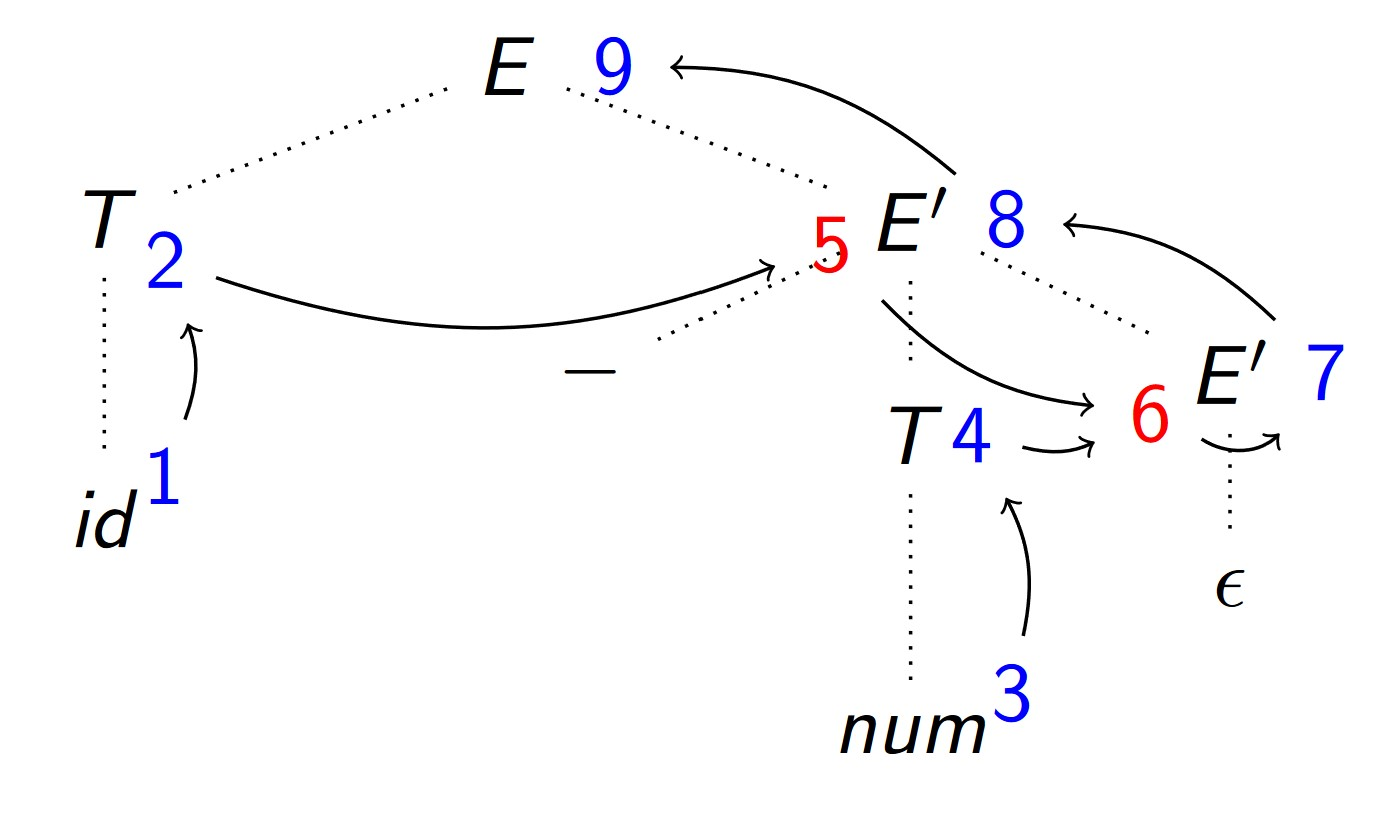
\includegraphics[width=.6\textwidth]{dependency-graph-ae-evaluation-order.jpg}
    \caption{Dependency Graph attributi ereditati con Evaluation Order}
    \label{fig:dependency-graph-ae-evaluation-order}
\end{figure}

Finalmente abbiamo la possibilità di osservare passo per passo come costruire il nostro abstract syntax tree seguendo l'evaluation order:

\begin{enumerate}
    \item recuperiamo le informazioni relativamente ad \(id\) (i.e. \(a\)) dalla symbol table mediante il riferimento presente in \(id.entry\);
    \item generiamo una foglia con etichetta \(id\) e un riferimento ad \(a\) nella symbol table), tale operazione viene eseguita dalla regola \(\{T.node = newLeaf(id, id.entry)\}\) per  \(T \to id\);
    \item recuperiamo il valore di \(num\) ottenuto dall'analisi lessicale mediante \(num.lexval\) (i.e. 4);
    \item generiamo la foglia per il valore di \(num\), tale operazione viene eseguita dalla regola \(\{T.node = newLeaf(num, num.lexval)\}\) per \(T \to num\);
    \item creiamo un riferimento alla foglia di \(a\) utilizzando la regola \(\{E'.i = T.node\}\) per  \(E \to TE'\). In questo passaggio dobbiamo recuperare \(T.node\) (che contiene un riferimento alle informazioni del sottoalbero sinistro) e assegnarlo a \(E'.i\), in modo che i passi successivi possano usufruirne;
    \item generiamo il nodo per la sottrazione \(a-4\): tale operazione viene eseguita dalla regola \(\{E_{1}'.i = newNode(-, E'.i, T.node)\}\) per \(E' \to -TE_{1}'\); anche in questo caso abbiamo bisogno di passare il riferimento ai passi successivi;
    \item creiamo un riferimento al nodo della sottrazione appena creato utilizzando la regola \(\{E'.node = E'.i\}\) per \(E' \to \varepsilon\);
    \item creiamo un riferimento allo stesso nodo utilizzando la regola \(\{E'.node = E_{1}'.node\}\) per \(E' \to -TE_{1}'\);
    \item infine creiamo un riferimento ancora allo steso nodo (esato, è proprio questo che si fa quando si ritorna da una ricorsione) utilizzando la regola \(\{E.node = E'.node\}\) per \(E \to TE'\).
\end{enumerate}

Il risultato finale è dunque rappresentabile nel seguente modo:

\begin{figure}[H]
	\centering
    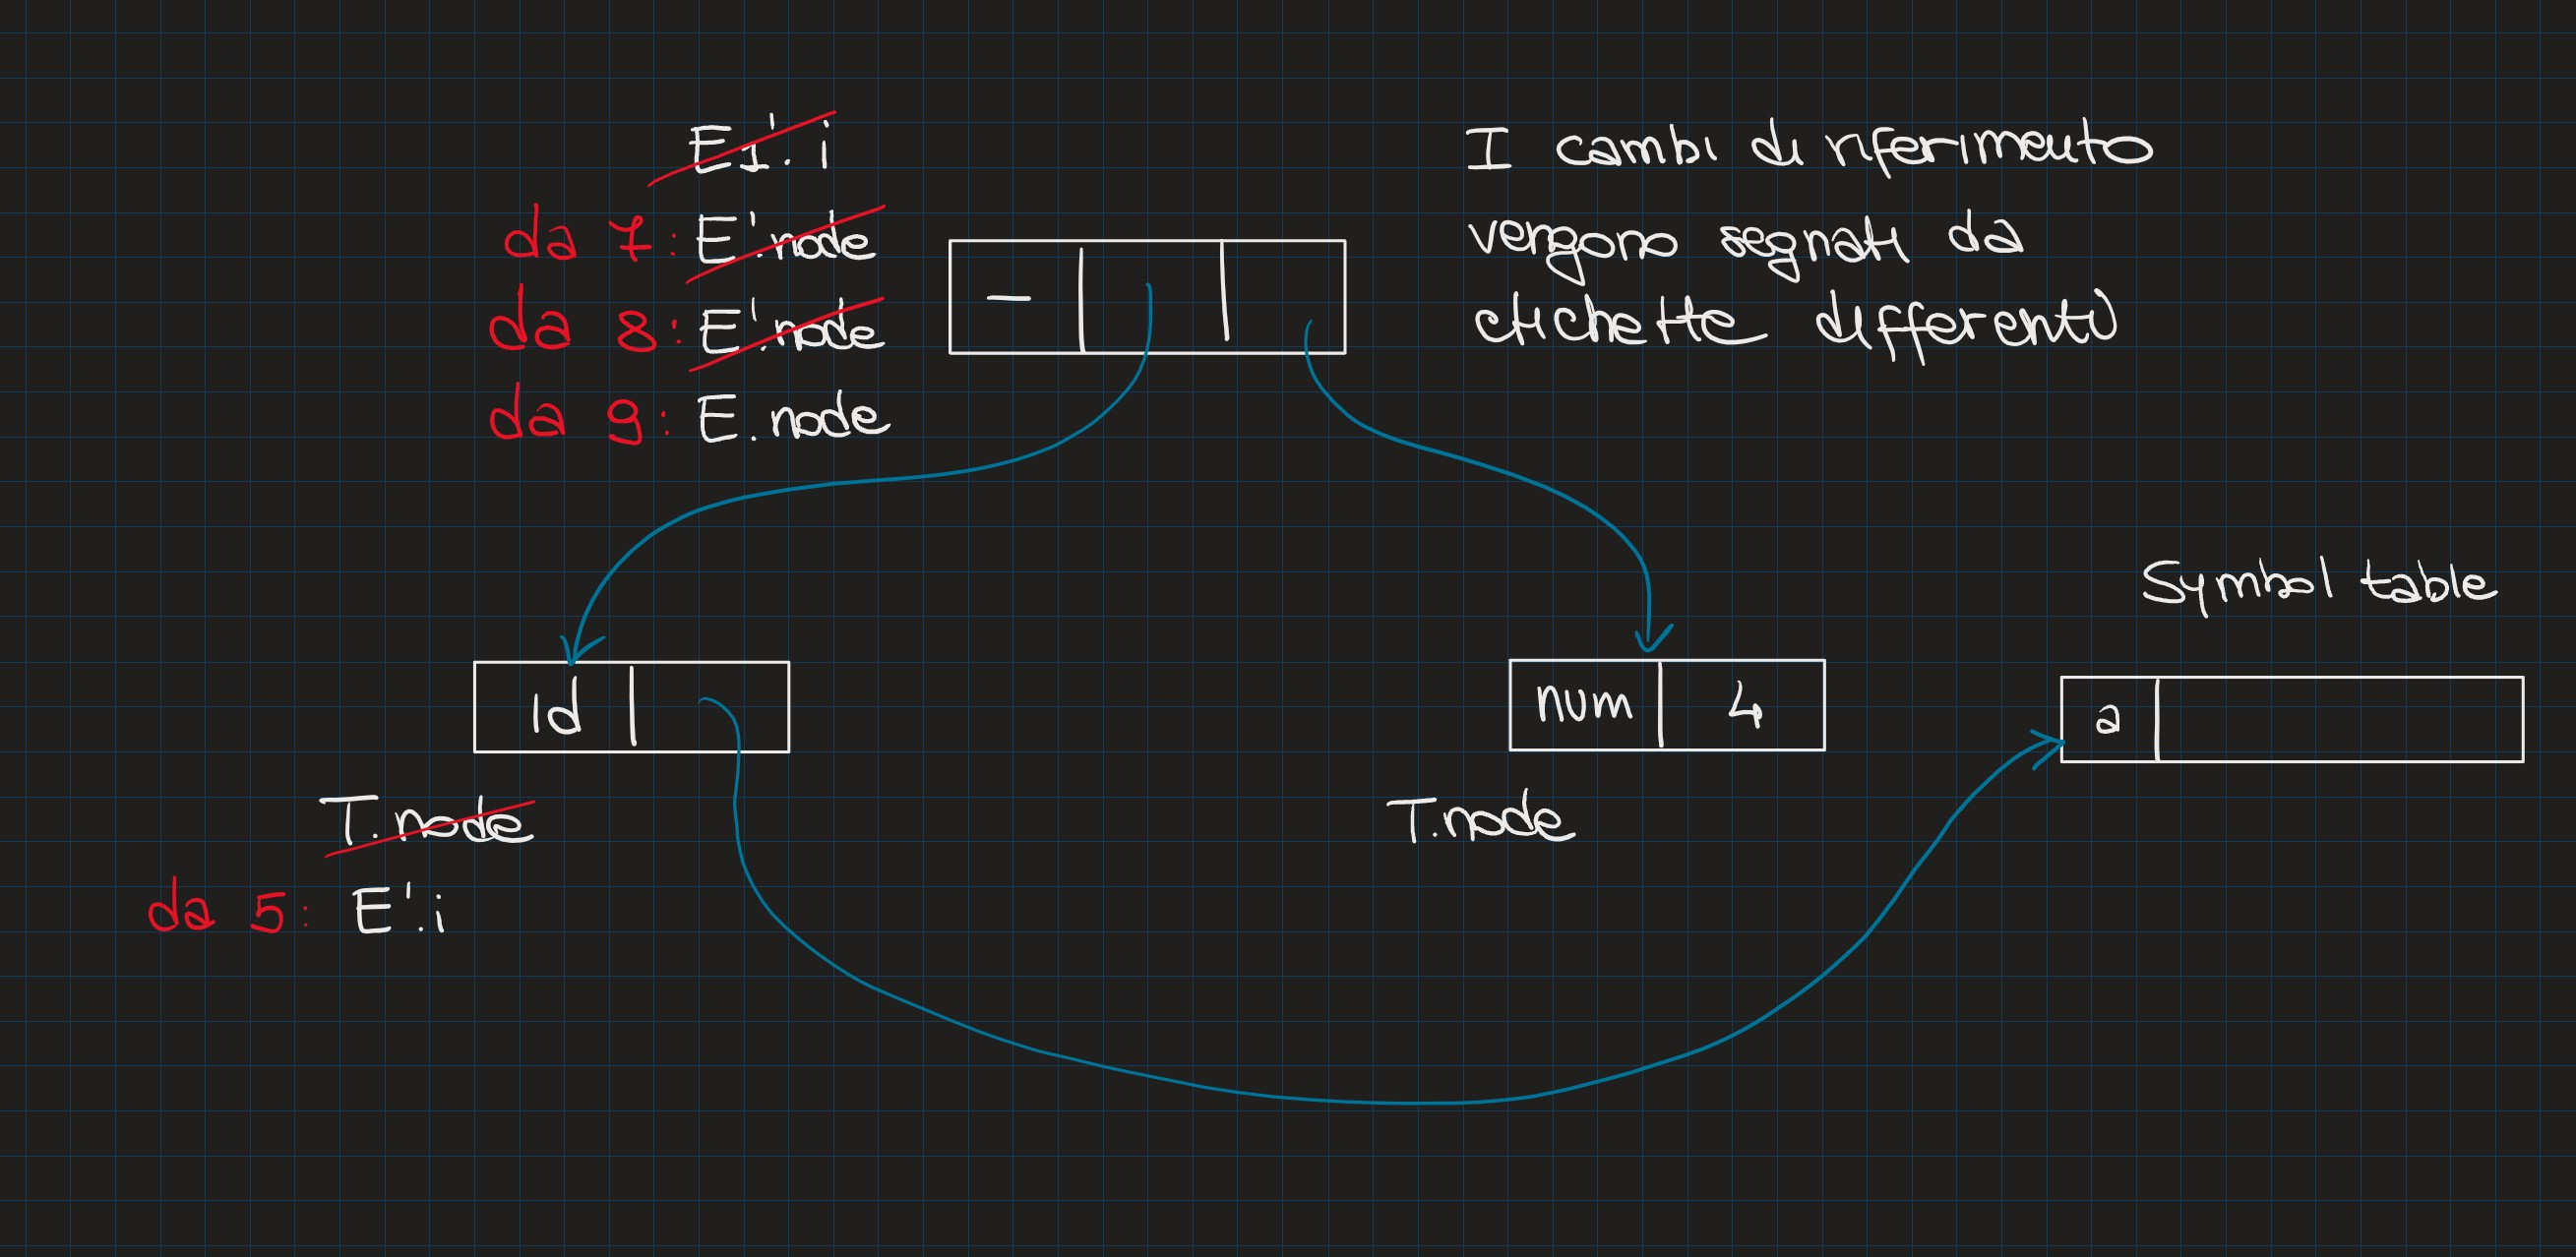
\includegraphics[width=.8\textwidth]{abstract-syntax-tree-ae.jpg}
    \caption{Abstract syntax tree attributi ereditati}
    \label{fig:abstract-syntax-tree-ae}
\end{figure}

\subsubsection{Es attribuzione tipo degli identificatori}

Consideriamo la seguente grammatica

\begin{align*}
    D &\to TL \\
    T &\to int \\
    T &\to float \\
    L &\to L_1, id \\
    L &\to id
\end{align*}

L'obbiettivo è quello di associare alle produzioni descritte delle regole per cui si possa aggiungere il tipo nella entry della symbol table degli identificatori dichiarati. Per poter aggionrare la tabella è necessario utilizzare la funzione \texttt{addtype(table\_entry, type\_instance)}.

Anche in questo caso partiamo da un esempio che può aiutarci per la definizione delle regole: supponiamo di avere la parola \emph{int id, id}, in questo caso per una derivazione leftomost i passi di derivazione che dobbiamo compiere sono

\begin{equation*}
    D \Rightarrow TL \Rightarrow int\; L \Rightarrow int\; L, id \Rightarrow int\; id, id
\end{equation*}

dunque il parse tree può essere così rappresentato

\begin{figure}[H]
	\centering
    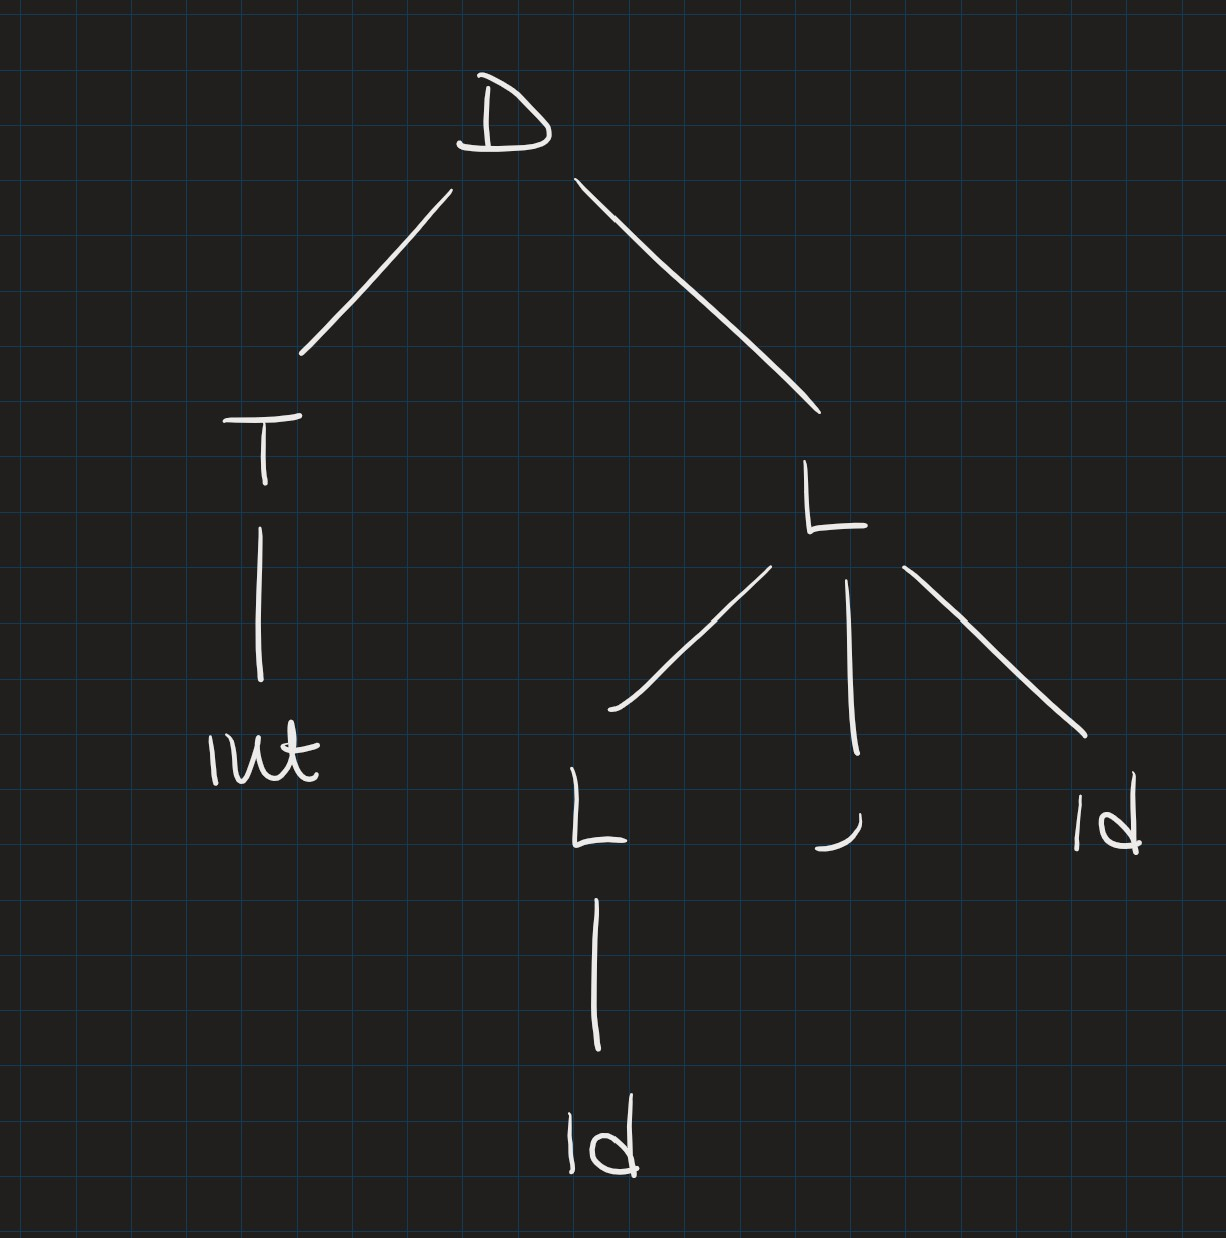
\includegraphics[width=.6\textwidth]{parse-tree-int-float.jpg}
    \caption{Parse tree aggiornamento tipo identificatori}
    \label{fig:parse-tree-int-float}
\end{figure}

Partiamo dalle produzioni più semplici, cioè quelle che si occupano di definire il tipo degli attributi: in questo caso banalmente possiamo passare l'attributo sintetizzato al driver della produzione

\begin{align*}
    T &\to int &\{T.type = int\} \\
    T &\to float &\{T.type = float\}
\end{align*}

Guardando il parse tree osserviamo che la risoluzione del sottoalbero destro dipende dal sottoalbero sinistro: una volta scoperto il tipo delle nostre entry abbiamo bisogno di fornire questa informazione alla funzione nell'altro sottoalbero, ma ciò è possibile solamente utilizzando degli attributi ereditati. Per questo motivo possiamo introdurre la seguente regola

\begin{align*}
    D &\to TL &\{L.i = T.type\} \\
\end{align*}

Una volta che abbiamo trovato il modo per poterci trasportare il tipo dobbiamo effettivamente utilizzarlo per le nostre entry: a questo scopo possiamo andare a valorizzare le regole per le produzioni rimaste nel seguente modo

\begin{align*}
    L &\to L_1, id &\{addtype(id.entry, L.i);\; L_1.i = L.i\}\\
    L &\to id &\{addtype(id.entry, L.i)\}
\end{align*}

Come è possibile notare, entrambe le produzioni le entry della tabella aggiungendo il tipo; nel primo caso viene aggiunta una regola per garantire la produzione degli attributi per i sottoalberi successivi.  
Riassumendo, le regole per la tipizzazione sono le seguenti:
\begin{align*}
    D &\to TL &\{L.i = T.type\} \\
    T &\to int &\{T.type = int\} \\
    T &\to float &\{T.type = float\} \\
    L &\to L_1, id &\{addtype(id.entry, L.i);\; L_1.i = L.i\}\\
    L &\to id &\{addtype(id.entry, L.i)\}
\end{align*}


\end{document}
